\documentclass[journal=jcim,manuscript=article]{achemso}

\usepackage[version=3]
{mhchem} % Formula subscripts using \ce{}

\usepackage{listings}
\usepackage{hyperref}
\usepackage{xr-hyper}
\usepackage{natbib}
\usepackage[newfloat]{minted}
\usepackage{multirow}
\usepackage{verbatim}

%% remove blank first page
% \usepackage{atbegshi}% http://ctan.org/pkg/atbegshi
% \AtBeginDocument{\AtBeginShipoutNext{\AtBeginShipoutDiscard}}

\externaldocument{SI}

\newenvironment{code}{\captionsetup{type=listing}}{}

\newcommand*\mycommand[1]{\texttt{\emph{#1}}}


\makeatletter
\let\oldminipage\minipage
\let\oldendminipage\endminipage
\renewenvironment{minipage}[1]{}{}
\g@addto@macro{\maketitle}{\let\minipage\oldminipage\let\endminipage\oldendminipage}
\makeatother

%%%%%
% fix the first page being blank and authors' affilliations clipping the second page
% how? adjusting font sizes doesn't work. 

%%%%%
%%%%%%%%%%%%%%%%%%%%%%%%%%%%%%%%%%%%%%%%%%%%%%%%%%%%%%%%%%%%%%%%%%%%%
%% Meta-data block
%% ---------------
%% Each author should be given as a separate \author command.

% fix some achemso rubbish
\renewcommand{\titlesize}{\Large}
\renewcommand{\affilsize}{\footnotesize	}
\renewcommand{\authorsize}{\footnotesize	}
\renewcommand{\emailsize}{\footnotesize}

%% Main manuscript contributors
\author{Hugo MacDermott-Opeskin}
\affiliation{Open Molecular Software Foundation, Davis CA, USA}
\author{Jenke Scheen}
\affiliation{Open Molecular Software Foundation, Davis CA, USA}
\author{Cas Wognum}
\affiliation{Valence Labs, Montréal, Québec, Canada}
\altaffiliation{Recursion Pharmaceuticals, Salt Lake City, UT, USA}
\author{Joshua, T Horton}
\affiliation{Open Molecular Software Foundation, Davis CA, USA}
\author{Devany West}
\affiliation{Open Molecular Software Foundation, Davis CA, USA}
\author{Alexander Matthew Payne}
\affiliation{Computational and Systems Biology Program, Memorial Sloan Kettering Cancer Center, New York, NY, USA}
\altaffiliation{Tri-Institutional PhD Program in Chemical Biology, Memorial Sloan Kettering Cancer Center, New York, NY, USA}
\author{Maria A Castellanos}
\affiliation{Computational and Systems Biology Program, Memorial Sloan Kettering Cancer Center, New York, NY, USA}
\author{Sean Colby}
\affiliation{Open Molecular Software Foundation, Davis CA, USA}

%% ASAP %%
\author{Edward Griffen}
\affiliation{MedChemica Consultancy Ltd, Macclesfield, UK}
\author{David Cousins}
\affiliation{MedChemica Consultancy Ltd, Macclesfield, UK}
\author{Jessica Stacey}
\affiliation{MedChemica Consultancy Ltd, Macclesfield, UK}
\author{Jasmin Cara Aschenbrenner}
\affiliation{Diamond Light Source, Didcot, UK}
\author{Daren Fearon}
\affiliation{Diamond Light Source, Didcot, UK}
\author{Blake Balcomb}
\affiliation{Diamond Light Source, Didcot, UK}
\author{Peter Marples}
\affiliation{Diamond Light Source, Didcot, UK}
\author{Charles W.E. Tomlinson}
\affiliation{Diamond Light Source, Didcot, UK}
\author{Ryan Lithgo}
\affiliation{Diamond Light Source, Didcot, UK}
\author{Max Winokan}
\affiliation{Diamond Light Source, Didcot, UK}
\author{Haim Barr}
\affiliation{Weizmann Institute of Science, Rehovot, IL}
\author{Noa Lahav}
\affiliation{Weizmann Institute of Science, Rehovot, IL}
\author{Gwendolyn Fate}
\affiliation{Thames Pharma Partners, USA}
\author{Bruce Lefker}
\affiliation{Thames Pharma Partners, USA}
\author{Ralph Robinson}
\affiliation{Thames Pharma Partners, USA}
\author{Tamas Szommer}
\affiliation{Centre for Medicines Discovery, Oxford, UK}
\author{Nick Lynch}
\affiliation{Curlew Research, UK}


%% OpenADMET
\author{Mallory Tollefson}
\affiliation{Open Molecular Software Foundation, Davis CA, USA}
\author{Cynthia Xu}
\affiliation{Open Molecular Software Foundation, Davis CA, USA}

% Valence 
\author{Jonny Hsu}
\affiliation{Valence Labs, Montréal, Québec, Canada}
\altaffiliation{Recursion Pharmaceuticals, Salt Lake City, UT, USA}
\author{Julien St-Laurent}
\affiliation{Valence Labs, Montréal, Québec, Canada}
\altaffiliation{Recursion Pharmaceuticals, Salt Lake City, UT, USA}
\author{Honore Etsmoberg}
\affiliation{Valence Labs, Montréal, Québec, Canada}
\altaffiliation{Recursion Pharmaceuticals, Salt Lake City, UT, USA}
\author{Lu Zhu}
\affiliation{Valence Labs, Montréal, Québec, Canada}
\altaffiliation{Recursion Pharmaceuticals, Salt Lake City, UT, USA}
\author{Andrew Quirke}
\affiliation{Valence Labs, Montréal, Québec, Canada}
\altaffiliation{Recursion Pharmaceuticals, Salt Lake City, UT, USA}

%% Participants
% All participants excluding the authors already listed in the main document
\author{Mohamed Iliyas Abdul Haleem}

\author{Irfan Alibay}
\affiliation{Open Molecular Software Foundation, Davis CA, USA}

\author{Gunjan Baid}
\affiliation{Inductive Bio, New York, NY, USA}

\author{Benjamin Birnbaum}
\affiliation{Inductive Bio, New York, NY, USA}

\author{Kevin Bishop}
\affiliation{Ontario Institute for Cancer Research, Toronto, ON, Canada}

\author{Hugo Bohorquez}
\affiliation{Ontario Institute for Cancer Research, Toronto, ON, Canada}

\author{Ashmita Bose}
\affiliation{University of Luxembourg, Luxembourg City, Luxembourg}

\author{C.J. Brown}
\affiliation{Alpha29, LLC}

\author{Jackson Burns}
\affiliation{MIT, Cambridge, MA, USA}

\author{Lianjin Cai}
\affiliation{University of Pittsburgh, Pittsburgh, PA, USA}

\author{Ruel Cedeno}
\affiliation{Novalix, 67000 Strasbourg, France}

\author{Vladimir Chupakhin}
\affiliation{Simulations Plus, Research Triangle Park, NC, USA}

\author{Finlay Clark}
\affiliation{Newcastle University, Newcastle, UK}

\author{Daniel Cole}
\affiliation{Newcastle University, Newcastle, UK}

\author{Carles Corbi-Verge}
\affiliation{Recursion, Salt Lake City, UT, USA}

\author{Muhammad Danial}
\affiliation{Shenzhen Institute of Synthetic Biology, Shenzhen Institutes of Advanced Technology, Chinese Academy of Sciences, Shenzhen 518055, China}

\author{Alec Davi}
\affiliation{Owkin, New York, NY, USA}

\author{Wim Dehaen}
\affiliation{UCT Prague, Prague, Czech Republic}

\author{Niklas Piet Doering}
\affiliation{Freie Universität Berlin, Berlin, Germany}

\author{Alexis Dougha}
\affiliation{BFA, Université Paris Cité, CNRS UMR 8251, Inserm U1133, 75013 Paris, France}

\author{Bryce Eakin}
\affiliation{Inductive Bio, New York, NY, USA}

\author{Anatol Ehrlich}
\affiliation{University of Vienna, Vienna, Austria}

\author{Rokas Elijosius} % [Pending check]
\affiliation{University of Cambridge, Cambridge, UK}

\author{Jozef Fülöp}
\affiliation{UCT Prague, Prague, Czech Republic}

\author{Anthony Gitter}
\affiliation{University of Wisconsin-Madison, Madison, WI, USA}
\altaffiliation{Morgridge Institute for Research, Madison, WI, USA}

\author{Yaowen Gu}
\affiliation{New York University, New York, NY, USA}

\author{Teresa Head-Gordon}
\affiliation{University of California, Berkeley, CA, USA}

\author{Ellena Jiang}
\affiliation{University of Vienna, Vienna, Austria}

\author{Benjamin Kaminow}
\affiliation{Computational and Systems Biology Program, Memorial Sloan Kettering Cancer Center, New York, NY, USA}

\author{Sina Khosravi}
\affiliation{Mashhad University of Medical Sciences, Mashhad, Khorasan Razavi, Iran}

\author{Asma Feriel Khoualdi} % [Pending check]
\affiliation{Newcastle University, Newcastle, UK}

\author{Eelke Bart Lenselink}
\affiliation{Galapagos NV, 2800 Mechelen, Belgium}

\author{Zhirong Liu}
\affiliation{Peking University, Beijing, China}

\author{Yue Liu}
\affiliation{University of Pittsburgh, Pittsburgh, PA, USA}

\author{Sijie Liu}
\affiliation{Freie Universität Berlin, Berlin, Germany}

\author{Yizhou Ma}
\affiliation{QuantaBricks, Newark, NJ, USA}

\author{Patrick Maher}
\affiliation{Inductive Bio, New York, NY, USA}

\author{Imke Mayer} % [Pending Check]
\affiliation{Owkin, New York, NY, USA}

\author{Antonia Mey}
\affiliation{University of Edinburgh, Edinburgh, Scotland, UK}

\author{Floriane Montanari} % [Pending check]
\affiliation{Owkin, New York, NY, USA}

\author{Taoyu Niu}
\affiliation{University of Pittsburgh, Pittsburgh, PA, USA}

\author{Ryusei Ogino}
\affiliation{Japan Tobacco INC., Minato City, Tokyo, Japan}

\author{Ashok Palaniappan}
\affiliation{SASTRA Deemed University, Thanjavur, Tamil Nadu 613401, India}

\author{Xiaolin Pan}
\affiliation{New York University, New York, NY, USA}

\author{Auro Patnaik}
\affiliation{University of Edinburgh, Edinburgh, Scotland, UK}

\author{Long-Hung Pham}
\affiliation{Imperial College London, London, UK}

\author{Luis Pinto}
\affiliation{Independent Researcher}

\author{Justin Purnomo}
\affiliation{University of California, Berkeley, CA, USA}

\author{Alexander Rich}
\affiliation{Inductive Bio, New York, NY, USA}

\author{Lars Schaaf}
\affiliation{University of Cambridge, Cambridge, UK}

\author{Christoph Schran}
\affiliation{University of Cambridge, Cambridge, UK}

\author{Satya Pratik Srivastava}
\affiliation{Shiv Nadar University, Greater Noida, Uttar Pradesh, India}

\author{Kunyang Sun}
\affiliation{University of California, Berkeley, CA, USA}

\author{Zhaoxi Sun}
\affiliation{Shenzhen University of Advanced Technology, Shenzhen, China}

\author{Valerij Talagayev}
\affiliation{Freie Universität Berlin, Berlin, Germany}

\author{Balamurugan Thirukonda Subramanian Balakrishnan}

\author{Alexandre Tkatchenko}
\affiliation{University of Luxembourg, Luxembourg City, Luxembourg}

\author{Wojtek Treyde}
\affiliation{University of Oxford, Oxford, UK}

\author{Austin Tripp}
\affiliation{Valence Labs, Quebec, Canada}

\author{Nopsinth Vithayapalert}
\affiliation{VISTEC, Pa Yup Nai, Thailand}

\author{Yingze Wang}
\affiliation{University of California, Berkeley, CA, USA}

\author{Azmine Toushik Wasi}
\affiliation{Shahjalal University of Science and Technology, Sylhet, Bangladesh}

\author{Steffen Wedig}
\affiliation{University of Cambridge, Cambridge, UK}

\author{Bofei Xu}
\affiliation{Peking University, Beijing, China}

\author{Weijun Zhou}
\affiliation{New York University, New York, NY, USA}



%% ASAP PIs
\author{Frank von Delft}
\affiliation{Diamond Light Source, Didcot, UK}
\author{Alpha Lee}
\affiliation{PostEra, Cambridge, MA, USA}
\author{Karla Kirkegaard}
\affiliation{Stanford University School of Medicine: Stanford, CA, US}
\author{Peter Sjö}
\affiliation{Drugs for Neglected Diseases initiative: Geneva, Genève, CH}

%% OpenADMET PIs
% \author{Sri Kosuri} 
% \affiliation{Octant Inc: Emeryville, CA, US}

\author{James S. Fraser}
\affiliation{University of California San Francisco, San Francisco, CA, USA}

%% John as final as PI across both
\author{John D. Chodera}
\affiliation{Computational and Systems Biology Program, Memorial Sloan Kettering Cancer Center, New York, NY, USA}

\email{*jenke.scheen@omsf.io}

% remove affil displaying
% \makeatletter
% \let\acs@address@list\relax
% \setlength\acs@space@post@address{0pt}
% \makeatother

%%%%%%%%%%%%%%%%%%%%%%%%%%%%%%%%%%%%%%%%%%%%%%%%%%%%%%%%%%%%%%%%%%%%%
%% The document title should be given as usual. Some journals require
%% a running title from the author: this should be supplied as an
%% optional argument to \title.
%%%%%%%%%%%%%%%%%%%%%%%%%%%%%%%%%%%%%%%%%%%%%%%%%%%%%%%%%%%%%%%%%%%%%
\title{A Computational Community Blind Challenge on Pan-Coronavirus Drug Discovery Data}

\begin{document}
%%%%%%%%%%%%%%%%%%%%%%%%%%%%%%%%%%%%%%%%%%%%%%%%%%%%%%%%%%%%%%%%%%%%%
%% The abstract environment will automatically gobble the contents
%% if an abstract is not used by the target journal.
%%%%%%%%%%%%%%%%%%%%%%%%%%%%%%%%%%%%%%%%%%%%%%%%%%%%%%%%%%%%%%%%%%%%%


\newpage

\begin{abstract}
Computational blind challenges offer critical, unbiased assessment opportunities to assess and accelerate scientific progress, as demonstrated by a breadth of breakthroughs over the last decade. We report the outcomes and key insights from an open science community blind challenge focused on computational methods in drug discovery, using lead optimization data from the AI-driven Structure-enabled Antiviral Platform (ASAP) Discovery Consortium's pan-coronavirus antiviral discovery program, in partnership with Polaris and the OpenADMET project. This collaborative initiative invited global participants from both academia and industry to develop and apply computational methods to predict the biochemical potency and crystallographic ligand poses of small molecules against key coronavirus targets, Severe Acute Respiratory Syndrome Coronavirus 2 (SARS-CoV-2) and Middle East Respiratory Syndrome Coronavirus (MERS-CoV) main protease (Mpro), as well as multiple ADMET assay endpoints, using previously undisclosed comprehensive experimental drug discovery datasets as benchmarks. By evaluating submissions across multiple tasks and compounds, we established performance leaderboards and conducted meta-analyses to assess methodological strengths, common pitfalls, and areas for improvement. This analysis provides a foundation for best practices in real-world machine learning evaluation, grounded in community-driven benchmarking. We also highlight how next-generation platforms, such as Polaris, enable rigorous challenge design, embedded evaluation frameworks, and broad community engagement. This paper reports the collective findings of the challenge, offering a high-level overview of the data, evaluation infrastructure, and top-performing strategies. We further provide context and support for the accompanying papers authored by the challenge participants in this special issue, which explore individual approaches in greater depth. Together, these contributions aim to advance reproducible, trustworthy, and high-impact computational methods in drug discovery, and to explore best practices and pitfalls in future blind challenge design and execution, including planned initiatives for the OpenADMET project.
\end{abstract}

%%%%%% MAKE THE WHOLE MANUSCRIPT DOUBLE COLUMN FOR EASIER FIGURE FORMATTING
% \twocolumn
%%%%%%%%%%%%%%%%%%%%%%%%%%%%%%%%%%%%%%%%%%%%%%%%%%%%%%%%%%%%%%%%%%%%%
%% INTRODUCTION
%%%%%%%%%%%%%%%%%%%%%%%%%%%%%%%%%%%%%%%%%%%%%%%%%%%%%%%%%%%%%%%%%%%%%
\section{Introduction}
%% DRUG DISCOVERY COMPCHEM DOESNT GET ENOUGH DATA FOR PROPER MODELS OR EVAL
Computational modeling for drug discovery is often hindered by data shortages, particularly in obtaining high-quality, openly accessible datasets that are sufficiently diverse to build useful predictive models as well as datasets representative of drug discovery campaigns useful for assessing real-world performance\cite{van_tilborg_deep_2024, volkamer_machine_2023}.  Predictive models, such as those used in structure-based drug design, molecular docking, and machine learning (ML), rely heavily on  large volumes of high-quality experimental data to be effective. However, much of this data remains proprietary, fragmented, or improperly reported, limiting model performance and reproducibility\cite{baker_1500_2016, ash_practically_2024, kapoor_leakage_2023, wognum_call_2024, volkamer_machine_2023}. Open-science initiatives that provide access to comprehensive datasets are crucial for advancing these models and improving their performance, as well as evaluating them under realistic conditions for prospective use.

%% TO BUILD PROPER MODELS WE NEED PROPER BENCHMARKS AND CHALLENGES
Beyond data availability, the development of sustainable and translatable computational models depends on robust strategies for objective evaluation of model performance\cite{wognum_call_2024, ash_practically_2024, kramer_need_2025}. Community blind challenges are especially well suited to this task providing a structured and impartial framework for method assessment. Crucially, participants in blind prospective modeling challenges do not have direct access to the test set, and receive only limited feedback on performance on this set over the course of the challenge. This reduces the risk of overfitting and ensures that the test set remains a close proxy for generalization. Blind challenges also enforce a separation between method development and method evaluation, minimizing the impact of evaluation errors and phenomena related to Goodheart's Law ("When a measure becomes a target, it ceases to be a good measure"; metric gaming, test set idiosyncrasies, cognitive biases, etc.)\cite{goodheart_types}. Several notable community blind challenges have driven progress in computational drug discovery: 
The \textit{CACHE Challenges}\cite{ackloo_al-awar_amaro_arrowsmith_azevedo_al._2022} evaluate prospective hit-finding methods by providing high quality experimental assessment of predictive hits for therapeutically relevant targets with little or no known chemical matter. Staged over a hit finding round and hit expansion round, CACHE has also fostered close collaboration between academia and industry in an open-science framework. The \textit{Drug Design Data Resource (D3R) Grand Challenges}\cite{parks_gaieb_chiu_yang_shao_walters_jansen_mcgaughey_lewis_bembenek_et} benchmarked pose prediction and binding affinity ranking algorithms (e.g., free energy calculation methods) using small, focused, and blinded protein–ligand datasets. The \textit{Statistical Assessment of Modeling of Proteins and Ligands (SAMPL)} Challenges\cite{sampl6_2018, sampl7_2022, sampl8_2022, sampl9_2024} focused model performance evaluation on a variety of tractable modeling bottlenecks relevant to drug discovery---physical properties, including partition/distribution coefficients (logP/logD), acid dissociation constant (pKa), and ligand hydration free energies, as well as protein-ligand and host-guest binding, over a series of challenges. The recent and innovative \textit{BELKA competition}\cite{quigley2024belka} tested participants ability to predict binding (categorically) using a very large DNA Encoded Library (DEL) dataset ($\sim$300M data-points), finding poor generalization to unseen scaffolds. Finally, the \textit{CASP competition}\cite{casp13_2019, casp14_2021, casp15_2023} challenged participants to predict protein structures \textit{a priori}, with famed breakthroughs by AlphaFold2 and RoseTTAFold transforming the computational drug discovery field\cite{jumper_evans_pritzel_green_figurnov_ronneberger_tunyasuvunakool_bates_žídek_2021, baek_2021}. However, most blind challenges to date have involved datasets either aggregated across drug discovery projects, often between different institutions and organizations or collected for the purposes of running a challenge. This creates a major gap in benchmarking how well current models perform on integrated 'real-world' drug discovery problems---i.e., involving the development of therapies against a defined biological target---and that span multiple assays relevant to a coherent Target Candidate Profile (TCP) such as biochemical and biophysical assays, Absorption, Distribution, Metabolism, Excretion, and Toxicity (ADMET), structural biology, and Pharmacokinetic—Pharmacodynamic (PKPD) experiments\cite{wognum_call_2024, volkamer_machine_2023}.


%% ASAP DISCOVERY RAN AS OPEN SCIENCE AND APPROACHED PRECLINICAL CANDIDATE DISCLOSURE MILESTONE - PERFECT OPPORTUNITY
During the SARS-CoV-2 pandemic, the COVID Moonshot consortium demonstrated the feasibility of developing a straight-to-generic main protease (Mpro) inhibitor in record time using an open-science approach\cite{boby_2023}. Building on this success, the AI-driven Structure-enabled Antiviral Platform (ASAP) Discovery Consortium (ASAP)\cite{ASAP_website} was launched as part of the National Institutes of Health (NIH) Antiviral Drug Discovery (AViDD) program\cite{AVIDD_niaid_2022}, leveraging structure-enabled and artificial intelligence (AI) approaches, alongside a global team of experts, to advance structural biology, medicinal chemistry, biochemistry, and pre-clinical development for antiviral drug discovery. One of the main pillars of ASAP is the organization's commitment to open science and global accessibility of antivirals through an equitable licensing structure\cite{griffen_2024}. ASAP's open-science approach requires regular disclosure of project data into the public domain (with some limitations around bleeding edge lead-optimization data), however, with ASAP's pan-coronavirus program (targeting SARS-CoV-2 and MERS-CoV Mpro\cite{sars_mers_tcp}) approaching a preclinical candidate disclosure in March 2025 (now disclosed)\cite{griffen_2025_acs}, a significant portion of its drug discovery data was withheld to ensure a successful patent application within ASAP's equitable-access intellectual property framework. This withheld dataset offered a unique opportunity to host a computational blind challenge to assess model performance on blinded real-world drug discovery data.


%% PARTNERSHIP WITH POLARIS AND OPENADMET%%
Running a computational blind challenge requires significant community engagement, technical expertise, and robust evaluation procedures. To this end, ASAP leveraged the Polaris platform \cite{wognum_call_2024, Polaris_website, wognum_polaris-hubpolaris_2025}, enabling open, easy access to ML-ready datasets and benchmarks in drug discovery. Polaris provides robust challenge infrastructure, dataset hosting in the cloud, and expertise in best practices for model evaluation. Polaris have also cultivated a passionate community of expert ML practitioners across academia and industry, lowering the barrier to engaging high quality participants. Additionally, ASAP partnered with OpenADMET, a new Advanced Research Projects Agency for Health (ARPA-H)\cite{ARPAH_website} funded consortium between the University of California San Francisco (UCSF), Octant Bio\cite{Octant_website}, and the Open Molecular Software Foundation (OMSF)\cite{OMSF_website}, focused on generating open data and models to enable accurate modeling of ADMET properties. The blind challenge developed by these partners will henceforth be referred to as the \textbf{ASAP-Polaris-OpenADMET antiviral competition}.


%% QUICK DESCRIPTION OF WHAT DATA WAS IN THE CHALLENGE
The dataset used in the challenge primarily consisted of real-world lead optimization (leadopt) data from the ASAP pan-coronavirus Mpro program, selected to mirror challenges faced in real-world lead optimization campaigns. To this end, three \textit{subchallenges} were chosen that reflected experimental processes common to drug discovery: 1) crystallographic ligand pose prediction, 2) biochemical potency prediction, and 3) ADMET endpoint prediction (Figure~\ref{fgr:datasets_overview}). Each of these subchallenges contained one or more endpoints (e.g MERS-CoV and SARS-CoV-2 Mpro potency for the potency subchallenge).


\begin{figure}
    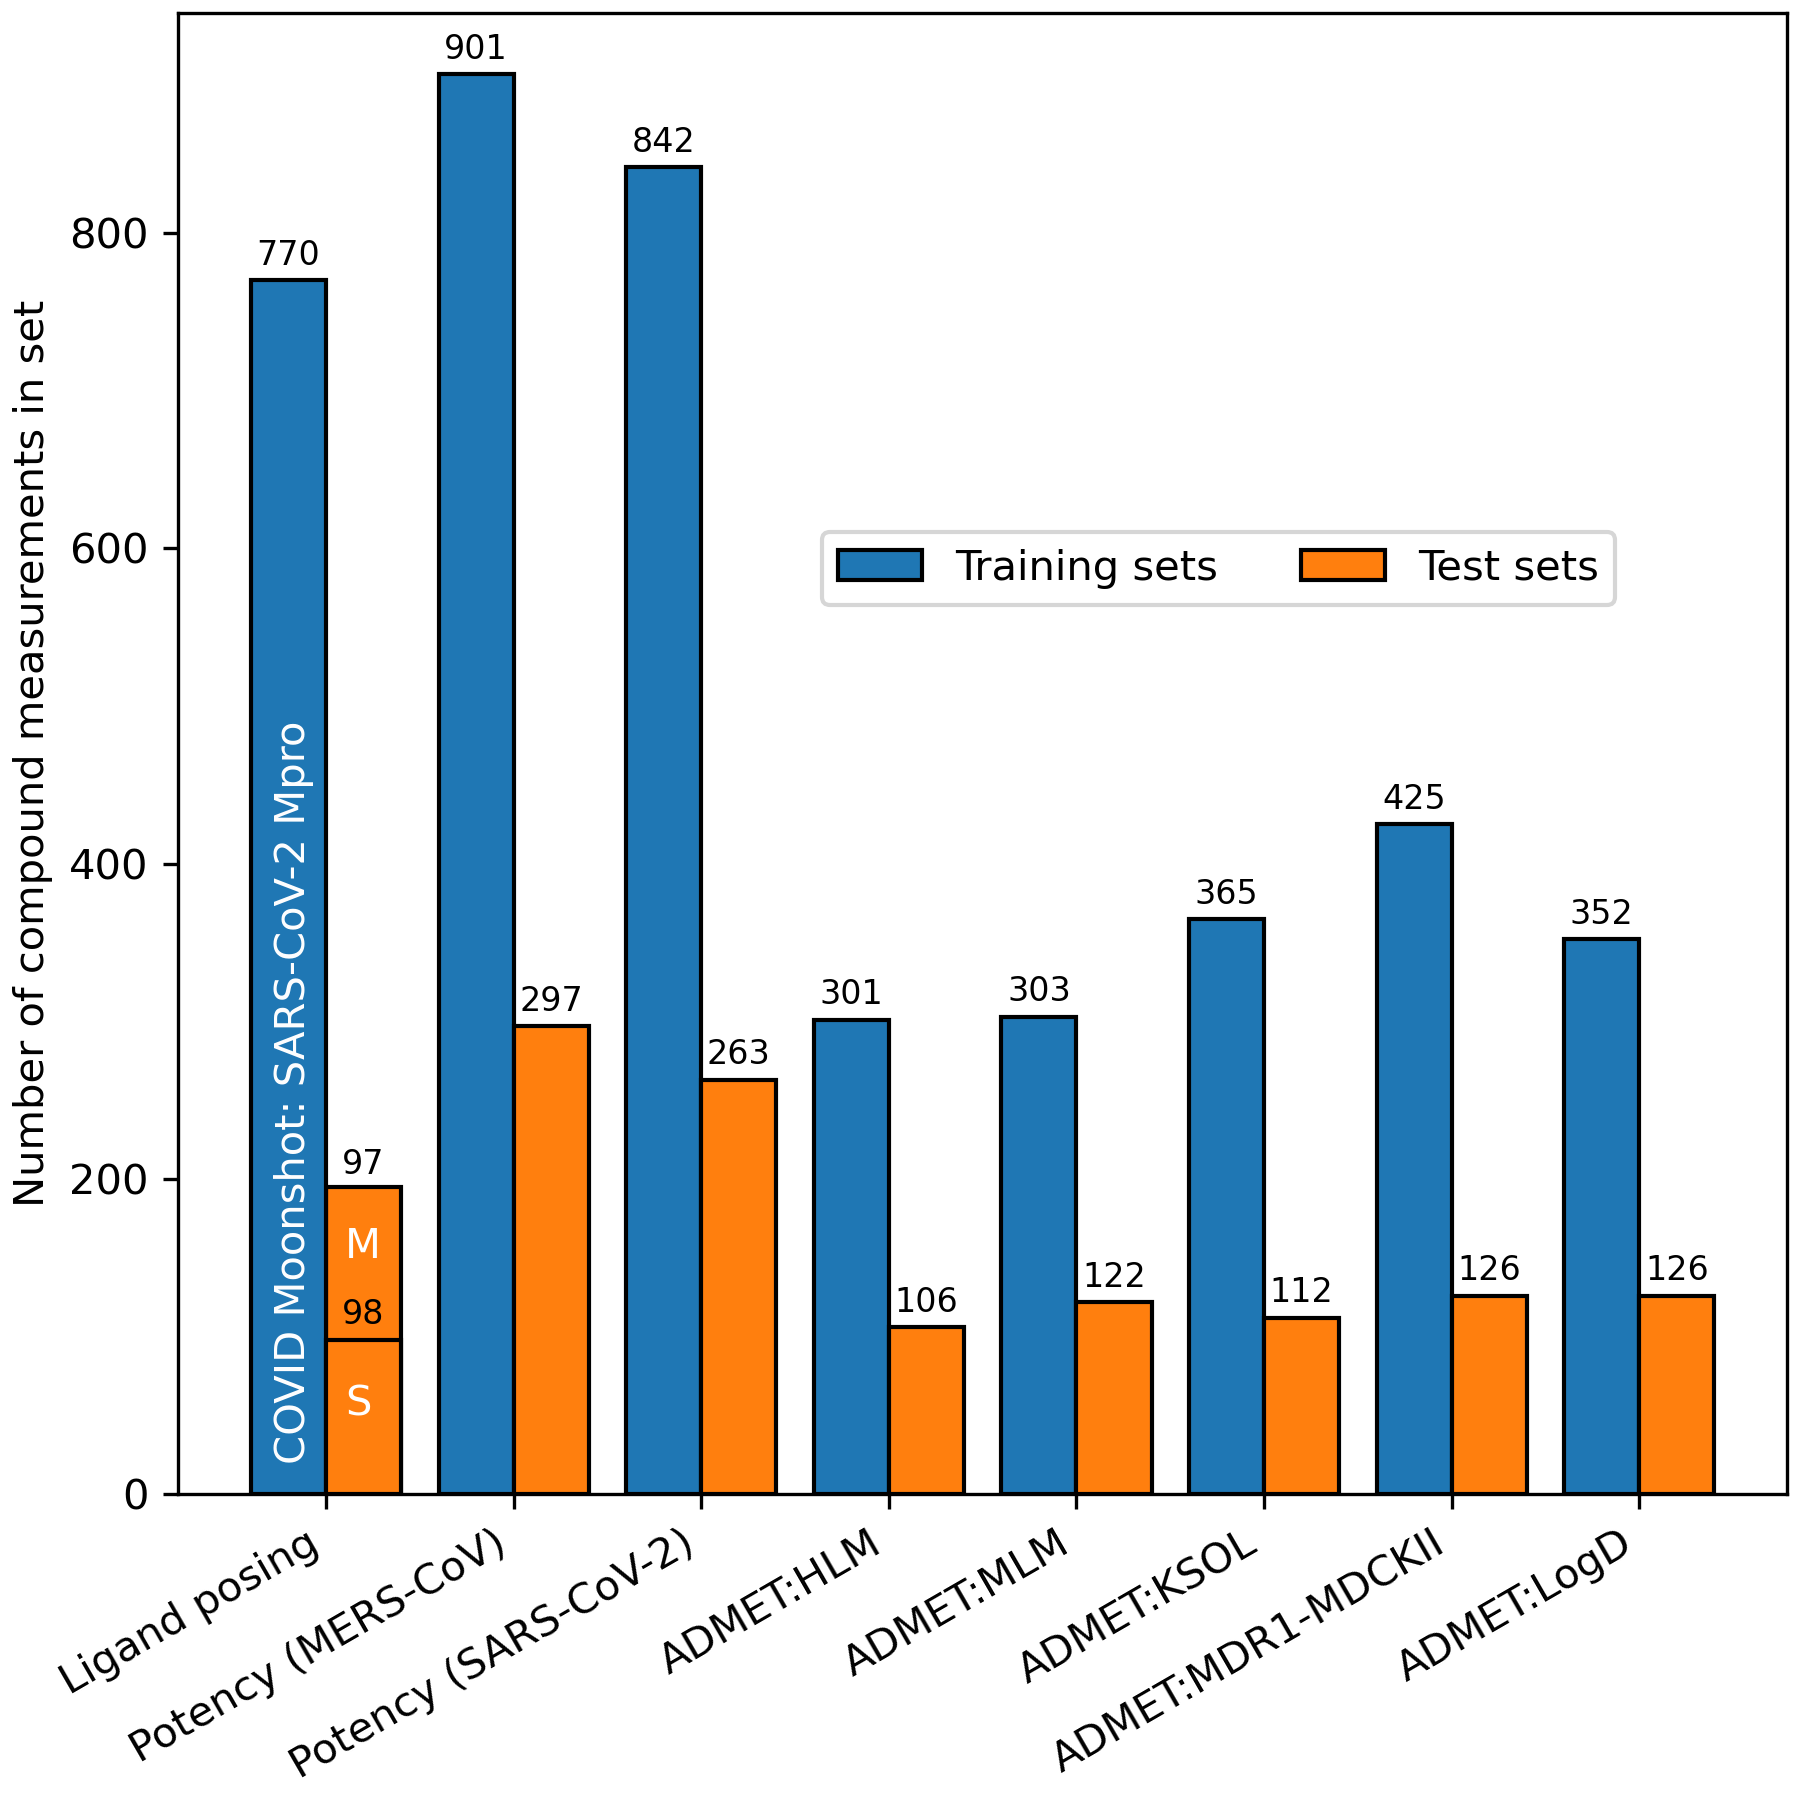
\includegraphics[scale=0.5]{01_figs_introduction/datasets_overview.png}
  \caption{\textbf{The ASAP-Polaris-OpenADMET blind challenge assessed predictive performance on lead optimization data temporally split into training and test sets.} 
  Final ML-ready training sets are shown as blue bars and test sets as orange bars with the total number of measurements annotated at the top of each bar. For the ligand posing subchallenge, \textbf{M} and \textbf{S} signify \textit{MERS-CoV Mpro} and \textit{SARS-CoV-2 Mpro} respectively. }
  \label{fgr:datasets_overview}
\end{figure}


%% MAIN OUTCOMES OF THE CHALLENGE
This paper summarizes the results of the challenge and contextualizes the accompanying papers in the Journal of Chemical Information and Modeling (JCIM) special issue, \textit{Open Science and Blind Data: The Antiviral Discovery Challenge}, in which selected participants each describe their approaches in greater detail. Overall, the challenge saw broad engagement with a global audience, including 381 challenge submissions across 66 unique participants, and with a total of 93 submissions for the final leaderboard. Significant post-challenge engagement was also observed, with robust scientific discussion during and after the challenge and several participating groups submitting their methods to the accompanying special issue. Broad, sustained engagement from industry and academia underscores the value of blind challenges as impartial benchmarks to drive future progress in computational drug discovery. 

The paper is organized as follows: we begin by describing the platform and overall challenge design, followed by details of the data collection and preparation process, including an example of challenge execution using the Polaris platform. We then outline the evaluation procedures and metrics used to assess performance. We conclude with a discussion of the main outcomes, key lessons learned, and prospects for future blind challenge implementations.

%%%%%%%%%%%%%%%%%%%%%%%%%%%%%%%%%%%%%%%%%%%%%%%%%%%%%%%%%%%%%%%%%%%%%
%% COMMUNITY
%%%%%%%%%%%%%%%%%%%%%%%%%%%%%%%%%%%%%%%%%%%%%%%%%%%%%%%%%%%%%%%%%%%%%
\section{Platform \& Community}

\subsection{Polaris provides a robust platform for benchmarking}

 Polaris provides a Python application programming interface (API)-based platform to enable easy access to drug discovery datasets and benchmarks. Serving as a common dataset curated according to best practices to avoid curation errors by individual organizations that may hinder method comparisons, Polaris enables access to ML-ready datasets and reproducible benchmarking\cite{Polaris_website, wognum_call_2024}. By enabling direct benchmark comparisons and minimizing the risk of data mishandling affecting results, modeling strategies can be evaluated consistently over time. Relative to similar platforms such as \href{kaggle.com}{Kaggle}, Polaris supports key modalities in drug discovery--including small molecules, proteins, and multi-omics data--and is designed with best practices tailored to each. Polaris' support for multiple drug discovery relevant modalities was critical for the multi-modal nature of the challenge.  Additionally, Polaris draws on the deep expertise of its advisory board, comprised of academic and industry leaders, to apply best practices in model evaluation and benchmarking\cite{ash_practically_2024}, which were employed throughout the challenge. Open, real-world benchmarks curated according to community-driven best practices hosted on Polaris contribute to trust in computational methods for drug discovery.

\subsection{Engaging the community}

Engaging the scientific community and attracting diverse participants across academia and industry is critical to running an impactful blind challenge. Polaris has built significant momentum around their platform and the dissemination of best practices for model evaluation and benchmarking\cite{wognum_call_2024}, actively engaging the community through a dedicated \href{discord.com}{Discord} server. To facilitate communication among participants, we created a specific Discord channel in the Polaris Discord server that participants used throughout the challenge for scientific and technical discussion. This provided a facile way for organizers to communicate with participants, and vice-versa, as well as for participants to assist each other and discuss results. While interactions preceded the official challenge start, and persisted beyond its close, the active portion of the challenge drove significant growth in overall engagement (Figure~\ref{fgr:timeline_engagement}A).

The challenge was designed to run in stages to maximize community engagement and allow feedback from participants. These stages were delineated by two intermediate leaderboards, allowing participants to gather feedback on the performance of their modeling strategies and provide feedback to organizers on challenge execution, such as possible modifications to evaluation metrics, and confusing data points. We also held office hours on two occasions, during which participants could engage with the experimentalists that generated the challenge data and ask in-depth questions of challenge organizers and experimentalists. The end of the challenge and final leaderboard was timed to coincide with the disclosure of the ASAP preclinical pan-coronavirus Mpro candidate at ACS Spring 2025\cite{griffen_2025_acs}, after which data could be freely unblinded. The full challenge timeline can be seen in Figure~\ref{fgr:timeline_engagement}B.

As part of our public outreach efforts, we ran an extensive social media campaign to promote both the office hours and the overall challenge, and organized a post-challenge symposium where top-performing participants presented their methodologies. A recording of the symposium is available on YouTube\cite{openadmet_asap_workshop}. 


\begin{figure}
    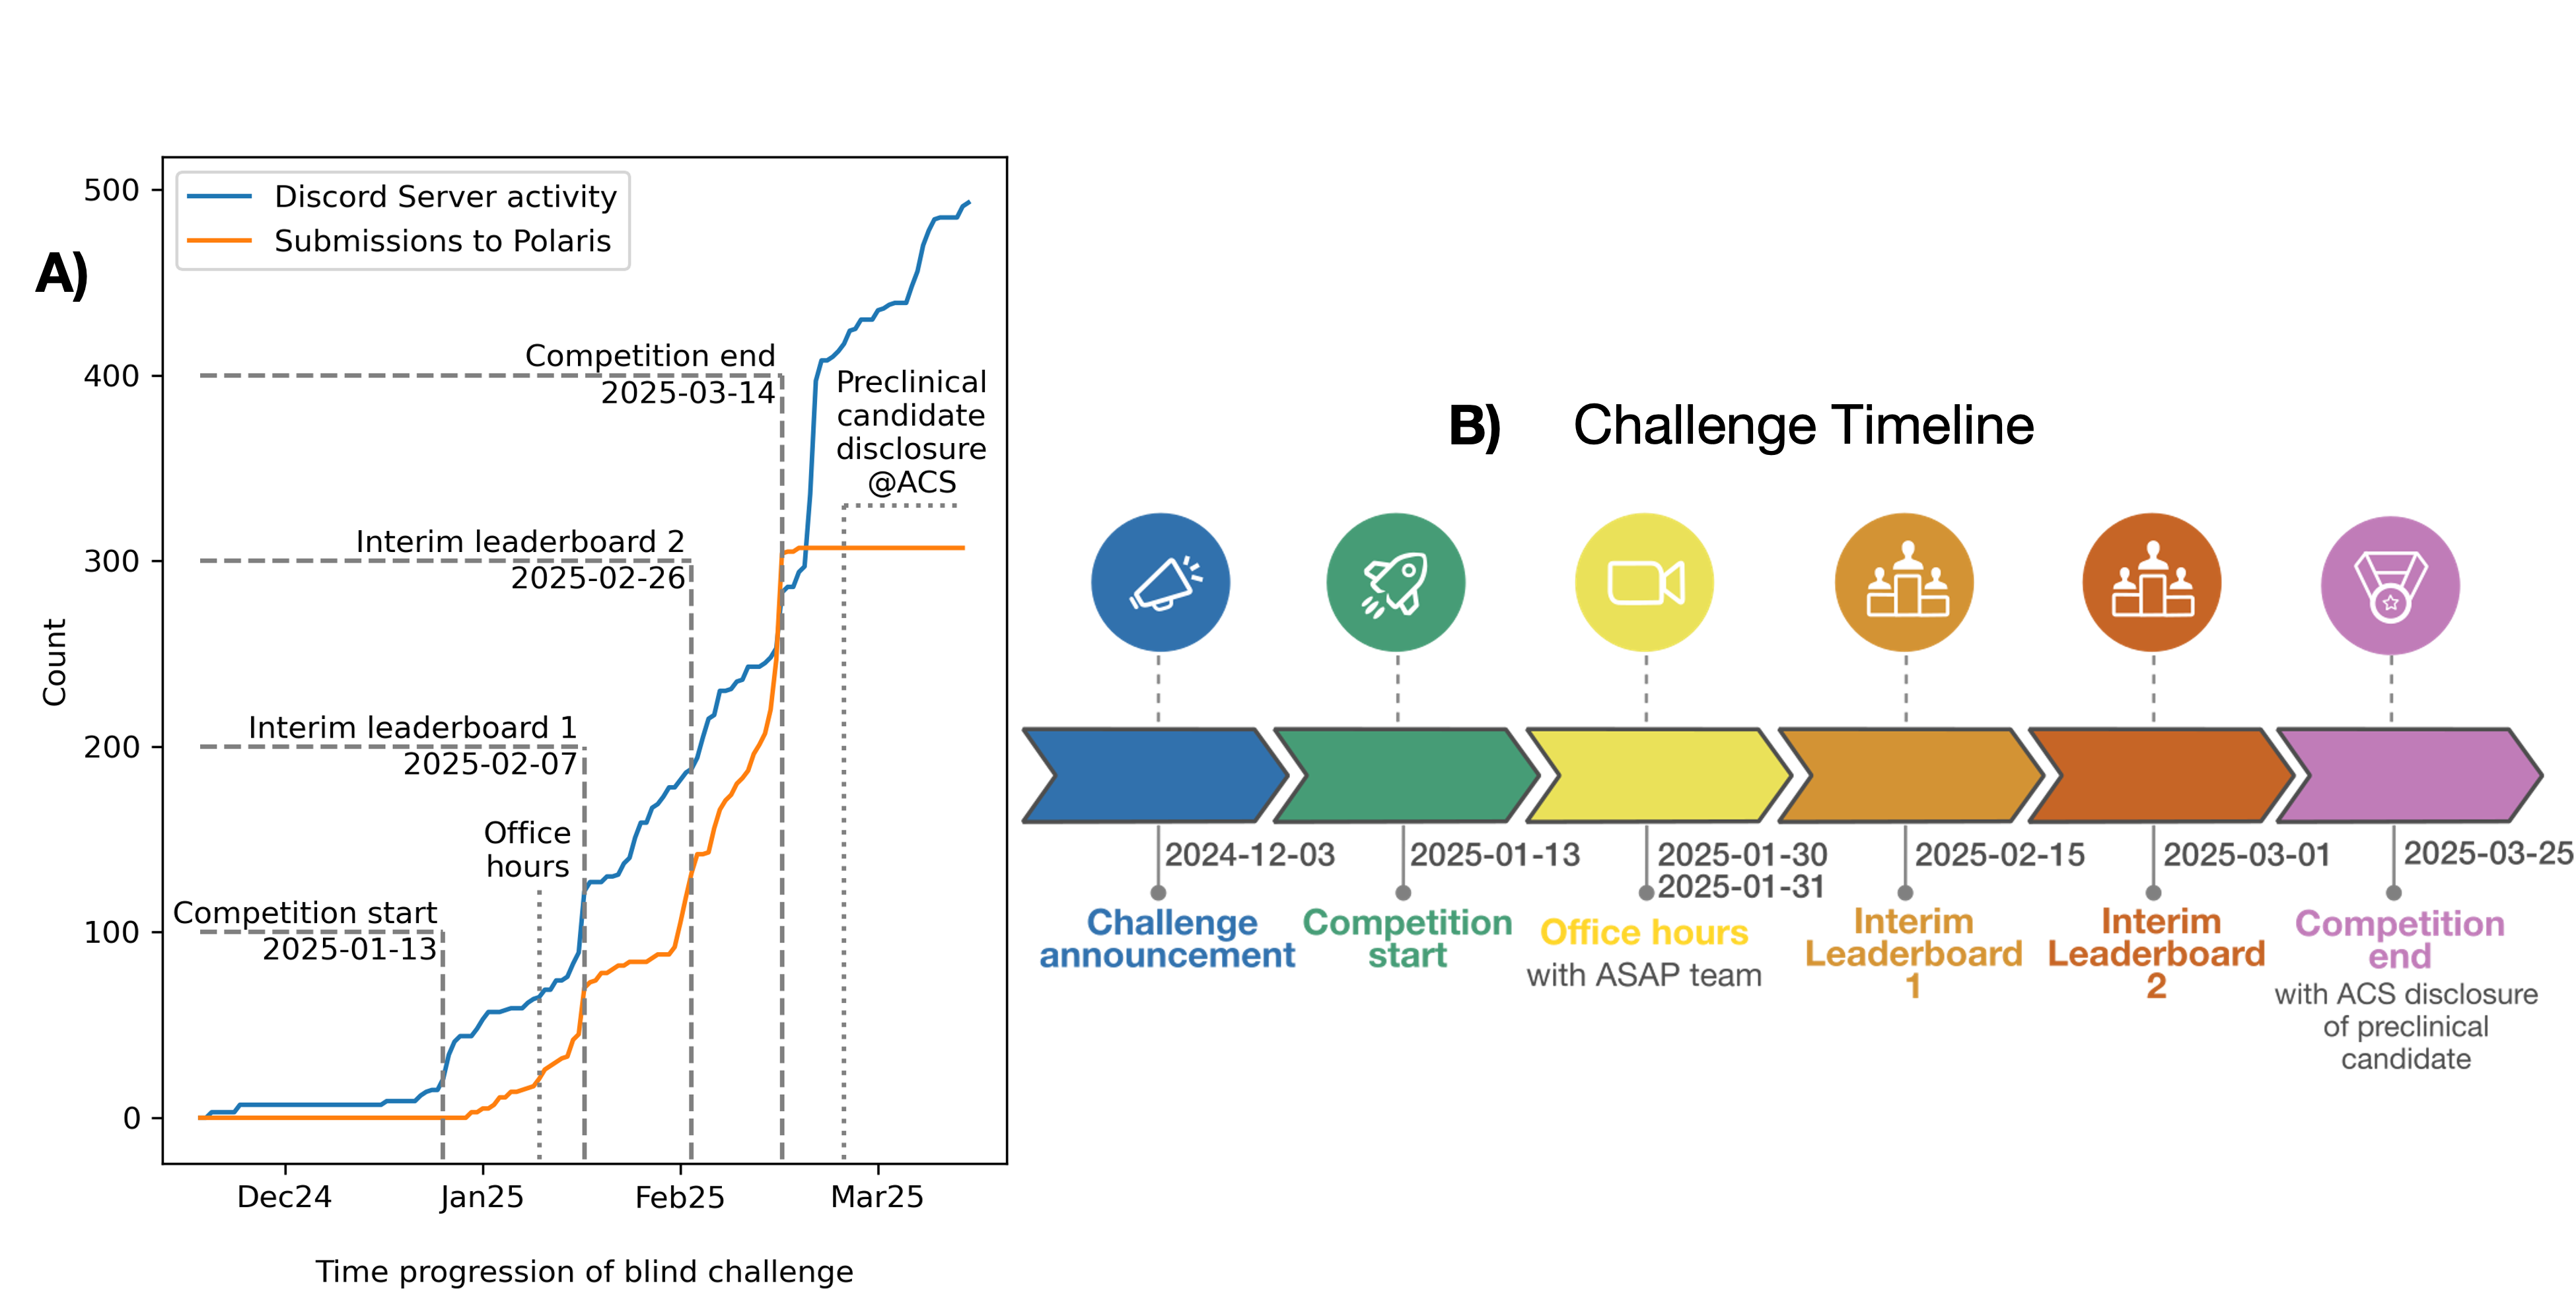
\includegraphics[scale=0.58]{02_figs_community/community_progress_and_timeline.png}
  \caption{\textbf{The ASAP-Polaris-OpenADMET Challenge spanned two months and saw a high volume of participation.} A) Community engagement for the blind challenge across its runtime with several milestones annotated with corresponding dates. Shown are the number of messages sent by participants over the Discord server in blue and the number of predictions submitted by participants to the Polaris platform in orange. Dotted lines indicate the virtual office hours that were hosted on 2025-01-30 and 2025-01-31 and the preclinical candidate disclosure at ACS on 2025-03-25; after this date all test set data was published. B) Schematic illustration of the timeline for the ASAP-Polaris-OpenADMET Challenge, with dates annotated.}
  \label{fgr:timeline_engagement}
\end{figure}

\begin{figure}
    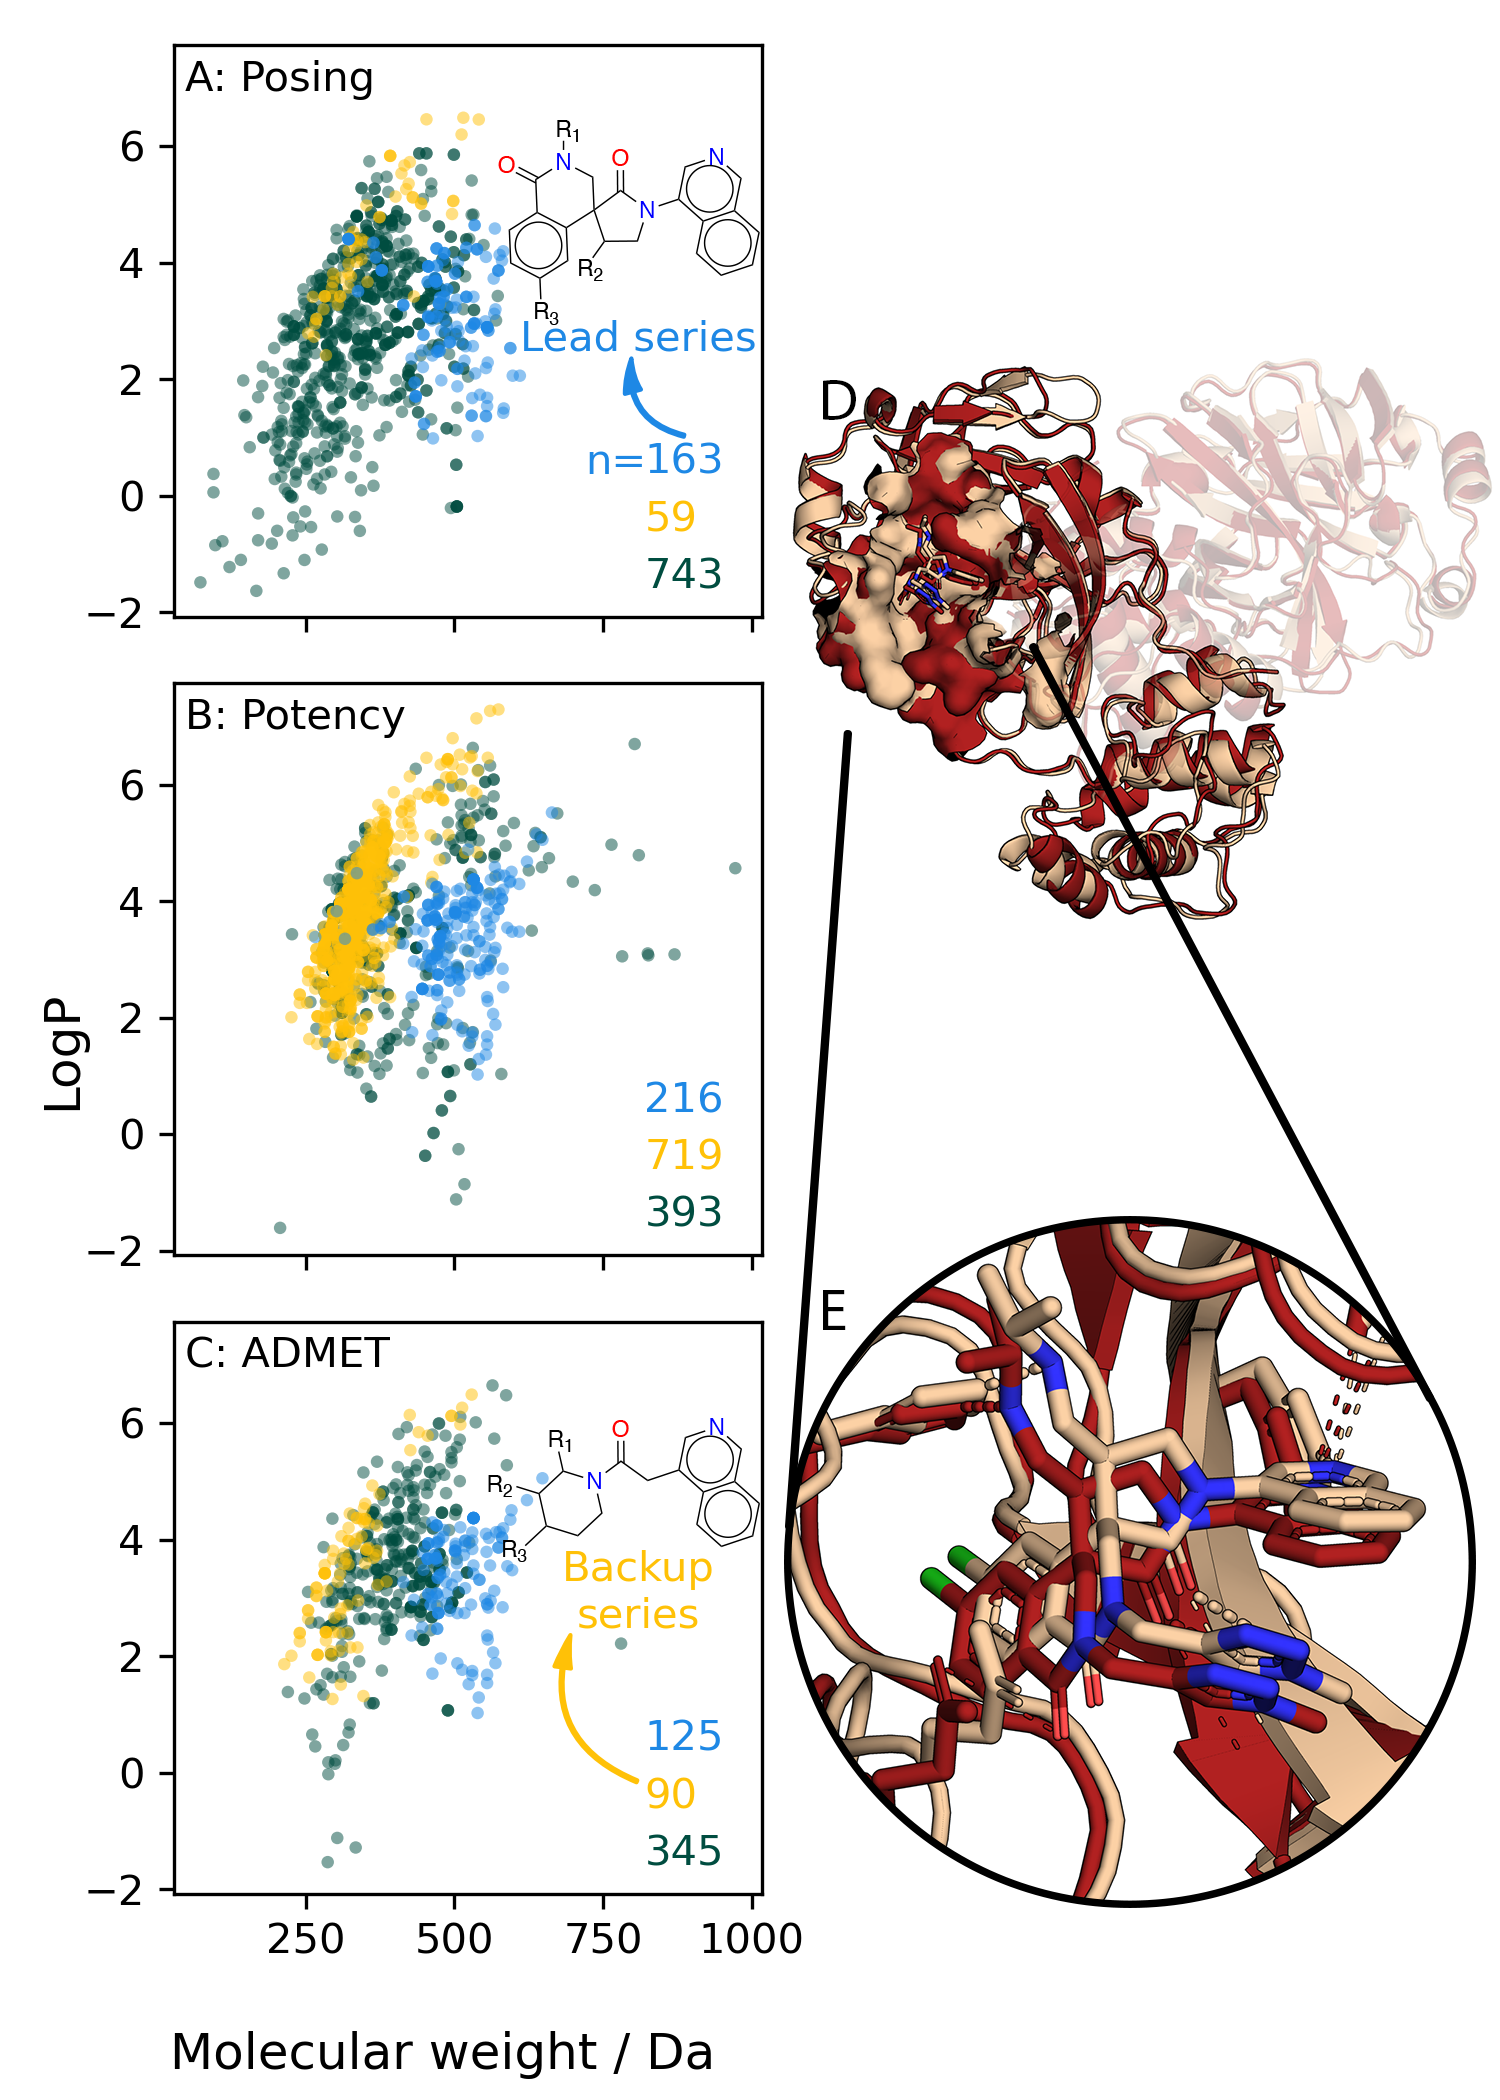
\includegraphics[scale=0.9]{03_figs_data_preparation/subchallenge_physprops_with_scaffolds.png}
  \caption{\textbf{Chemical matter used in each subchallenge spans multiple chemical series of multiple chemical property characteristics.} These plots show the lead series (blue) that progressed to preclinical candidate nomination, a backup series (yellow) and any miscellanous compounds (green). The different subchallenges that the compounds were involved in are annotated on the three panels (A/B/C). The right-hand-side panels show the SARS-CoV-2 Mpro (red) and MERS-CoV Mpro (cream) with ASAP-0017445 X-ray structures in the system dimer form with chain B semi-opaque (D) and a blowup of the active site of both targets with each X-ray pose of ASAP-0017445 shown with contacts colored per corresponding target (E). }
  \label{fgr:physprops_scaffolds}
\end{figure}

%%%%%%%%%%%%%%%%%%%%%%%%%%%%%%%%%%%%%%%%%%%%%%%%%%%%%%%%%%%%%%%%%%%%%
%% DATA PREPARATION AND EVALUATION
%%%%%%%%%%%%%%%%%%%%%%%%%%%%%%%%%%%%%%%%%%%%%%%%%%%%%%%%%%%%%%%%%%%%%
\section{Data Preparation \& Evaluation of Models}

Data was collated from ASAP Discovery’s pan-coronavirus Mpro inhibitor program (spanning both SARS-CoV-2 Mpro and MERS-CoV Mpro), which at the time of challenge initiation had successfully reached preclinical candidate nomination. Available data concerned three aspects: in-vitro biochemical potency measurements, ADMET properties, and structural biology (X-ray crystallography) across the two protein targets. Chemical matter for the challenge was organized into three series: the nominated spirolactam containing \textit{lead} series, a \textit{backup} series, and compounds that could not be readily assigned to either series via Bemis-Murcko scaffolds\cite{bemis_murcko_1996} (Figure~\ref{fgr:physprops_scaffolds}).

As part of its pandemic preparedness mission, ASAP Discovery has pursued an open-science policy in conjunction with an IP strategy designed to ensure equitable and affordable global access to any derived therapeutics. This is achieved through phased open science in the early stages of drug discovery, followed by time-limited confidentiality in later stages of leadopt, and “minimally defensive patenting” for candidate molecules\cite{griffen_2024}. Practical implications for the challenge were that molecules previously disclosed as part of our open-science efforts and those sufficiently congeneric (could be construed as \textit{prior art}\cite{ACS_patents}) to molecules claimed in a minimally defensive patent (filed, but not yet disclosed at the time of the challenge) could not be included in the challenge data.

\subsection{Reference data collection}

Mpro inhibition was measured via a direct \textit{in vitro} dose-response biochemical assay, using a fluorescent Mpro substrate. Experiments were performed primarily at the Weizmann Institute of Science. Technical differences between the assays for SARS-CoV-2 Mpro\cite{sars_mpro_dose_response_protocol} and MERS-CoV Mpro\cite{mers_mpro_dose_response_protocol} are explored in their respective protocols available online (along with many others) at the ASAP protocols.io\cite{asap_protocols_io}. Following data collection, half maximal inhibitory concentrations (IC50s) were determined by fitting to dose response curves. The fitting procedure differed between SARS-CoV-2 Mpro and MERS-CoV Mpro due to differences in binding kinetics between the two proteins, both of which are homodimeric but differ in their association constants. SARS-CoV-2 Mpro used a traditional fit to the Hill equation\cite{Hill_eq_1910} with a four-parameter logistic function. For MERS-CoV Mpro, the weakly bound dimer can undergo ligand-induced dimerisation and an alternative curve fitting procedure used to account for the resulting low concentration activation. Challenge data used pIC50s (log10 IC50), as calculated from the raw IC50 values pooled from replicates. 

SARS-CoV-2 Mpro and MERS-CoV Mpro proteins were expressed and purified by the Centre for Medicines Discovery at the University of Oxford. Crystal constructs were created and soaked with compounds and analyzed at the X-ray beamline at Diamond Light Source according to the two protocols outlined for SARS-CoV-2 Mpro\cite{sars_mpro_crystal_protocol} and MERS-CoV Mpro, respectively\cite{mers_mpro_crystal_protocol}. 

ADMET data was collected on an ADMET panel from Bienta specifically for the goals of the pan-coronavirus Mpro program as defined in ASAP’s Target Candidate Profile\cite{sars_mers_tcp}. This consisted of five primary endpoints: Mouse Liver Microsomal (MLM) intrinsic clearance ($CL_{int}$), Human Liver Microsomal (HLM) intrinsic clearance ($CL_{int}$) \cite{hlm_mlm_assay_protcol}, Kinetic Solubility (KSOL)\cite{ksol_assay_protocol}, LogD as a measure of lipophilicity\cite{logD_assay_protocol}, and a cell permeability assay (Perm) in p-glycoprotein expressing Madin-Darby canine kidney cells (MDR1-MDCKII cells)\cite{perm_assay_protocol}. For the cell permeability assay, the apical to basolateral apparent permeability was used as the primary endpoint.

\begin{table}[ht]
\centering
\caption{Summary of Endpoints by subchallenge}
\begin{tabular}{|l|l|l|}
\hline
\textbf{subchallenge} & \textbf{Endpoint} & \textbf{Units} \\
\hline
\multirow{2}{*}{Potency} 
& SARS-CoV-2 Mpro pIC50 & unitless (log scale) \\
& MERS-CoV Mpro pIC50    & unitless (log scale) \\
\hline
\multirow{2}{*}{Ligand pose} 
& SARS-CoV-2 Mpro liganded crystal structures & NA \\
& MERS-CoV Mpro liganded crystal structures   & NA \\
\hline
\multirow{5}{*}{ADMET} 
& Mouse Liver Microsomal $CL_{int}$ (MLM)  & uL/min/mg \\
& Human Liver Microsomal $CL_{int}$ (HLM)  & uL/min/mg \\
& Kinetic Solubility (KSOL)               & µM \\
& LogD                                    & unitless (log scale) \\
& Cell permeability (apical-to-basolateral, MDR1-MDCKII cells) & 10\textsuperscript{-6} cm/s \\
\hline
\end{tabular}
\end{table}

\subsection{ML-ready dataset preparation}

Data was collated from ASAP’s Collaborative Drug Discovery (CDD, collaborativedrug.com) vault, a research informatics database platform that aggregates assay outcomes by molecule. Data was split into a training set that was released to participants and a blind test set that participants were evaluated on. A target 75:25 train:test split was selected for the ADMET and potency prediction challenges, while for the pose prediction challenge data from the COVID Moonshot\cite{boby_2023} (also solved by X-ray crystallography at Diamond Light Source) was used as the training set totaling 770 structures for SARS-CoV-2 Mpro only, while the test set comprised 98 SARS-CoV-2 Mpro structures and 97 MERS-CoV Mpro structures from the ASAP Discovery Consortium (See Figure \ref{fgr:datasets_overview}).  

For the ADMET and potency subchallenges we used a temporal split of the data to create a challenge more representative of real-world drug discovery, where molecules must be evaluated prospectively\cite{sheridan_time-split_2013}. However, this had to be balanced against minimization of leakage between endpoints, which could jeopardize competition integrity by revealing test set molecules to participants in the training set of other endpoints. This was particularly challenging for the ADMET subchallenge, in which several endpoints have limited amounts of data, meaning that a multi-endpoint, multi-subchallenge split had to be carefully designed to minimize leakage between endpoints and subchallenges. 

To balance these competing concerns, the following hybrid splitting procedure was followed for the ADMET and potency subchallenges. First, all molecules in common between both the ADMET and potency subchallenge were determined (N=197). The split for each endpoint that minimizes leakage across all endpoints and datasets will contain as many of the shared molecules as possible in the \textbf{test set} such that the test set can "hold out" as many structures as possible across the totality of compounds. For the potency subchallenge, this was achieved by first placing the common molecules in the test set and then adding remaining molecules newest-first by MERS-CoV Mpro potency assay date to the test set such such that the test set is biased towards newer compounds (simulated time based split). This split (common augmented with MERS-CoV Mpro date-ordered) was then used to split the SARS-CoV-2 data. MERS-CoV Mpro potency assay date was chosen to bias the time based element of the split as, generally speaking, MERS-CoV Mpro assays were enabled after SARS-CoV-2 Mpro assays, providing a better bias towards newer compounds. Note that in this splitting procedure, tradeoff between leakage and split ratios results in the elimination of leakage \textit{within the potency challenge}, but with some variation in the exact 75:25 train-test split ratio by endpoint (SARS-CoV-2 Mpro pIC50 vs MERS-CoV Mpro pIC50). Overall this procedure can be thought of as a leakage-minimizing, date-biased split for a single endpoint (e.g MERS-CoV Mpro pIC50), with the other endpoint(s) split using the same indices.

A similar procedure was followed for the ADMET subchallenge, however the number of common molecules that would need to be placed in the test set grossly exceeds the 75:25 train-test ratio for some endpoints (Figure \ref{fgr:datasets_overview}). To minimize the impact of this while still biasing by date, the common molecules were ordered by LogD assay date and selected to satisfy a 75:25 train test split. The LogD time-based split was used to also split the other endpoints such that a consistent split was shared by the ADMET endpoints, eliminating between-endpoint leakage \textit{within the ADMET subchallenge} and biasing by date while also maximizing the number of common molecules held out between the potency and ADMET sets. Given the dataset sizes and extent of overlap there is an unavoidable ~70 compounds leak between the ADMET training set and potency test set (common molecules that were not be placed in the ADMET test set). However this between-endpoint leakage is not expected to provide significant information gain to the participants given that the leaked subset cannot be known \textit{a-priori}.

The data was then cleaned to be ML-ready according to the following steps. Compounds marked as below or above assay detectable range with a ChEMBL\cite{zdrazil_2024_chembl}-style modifier (i.e., $<$, $<=$, $>=$, $>$) were removed. Duplicate molecules were removed, with some missed on an an initial pass and removed following detection on by participants. Where a molecule had data recorded for an endpoint more than once, the most recent data collection was selected. Datasets with out-of-range datapoints and some additional endpoint-specific assay data were made available for the participants in case they wanted to leverage the additional negative data in their models. The final ML-ready datasets were uploaded to the Polaris platform, with each subchallenge represented as a multitask matrix. See Figure \ref{fgr:datasets_overview} for an overview of the datasets available. 

\subsection{Running the challenge on the Polaris platform}

Participants uploaded their predictions to the Polaris platform via the API over the course of the challenge. Example Python code detailing how participants were expected to submit their predictions is shown in Listing \ref{code:submission}. This provides significant operational advantages relative to modes of running other challenges, which include large amounts of manual data handling. A consistent Pythonic API also allows participants to colocate their modeling efforts with submission to the challenge infrastructure, e.g. in a Jupyter notebook\cite{kluyver_2016_jupyter}, enhancing reproducibility.

\begin{code}
\setminted{baselinestretch=0.5} % decreases vertical spacing between lines
\captionof{listing}{Example Python code to submit to Polaris API}
\label{code:submission}
\begin{minted}{python}
import polaris as po

# Load the competition data from the Polaris platform and split it
competition = po.load_competition("asap-discovery/antiviral-potency-2025")
train, test = competition.get_train_test_split()

# Make predictions
y_pred = my_participant_model(test)

# Submit predictions to the Polaris platform
competition.submit_predictions(
    predictions=y_pred,
    prediction_name="my-predictions",
    prediction_owner="participant_name",
    report_url="https://www.my_report.com",
)
\end{minted}
\end{code}


To enable participants to easily use the Polaris challenge infrastructure, we provided example notebooks with baseline models to demonstrate how to submit to each of the subchallenges (see Evaluation Procedure). These were made available on GitHub (https://github.com/asapdiscovery/asap-polaris-blind-challenge-examples). 

While evaluation of tabular data submissions for the potency and ADMET subchallenges did not pose any technical difficulties, the ligand pose subchallenge proved more complex. Due to technical constraints on storage and bandwidth in the Polaris backend, we could not store and evaluate submissions of full protein-ligand structures for each molecule for each participant. Instead, participants were required to submit a serialized RDKit molecule of the ligand only, pre-aligned to a reference structure (reference code provided in examples). While circumventing technical issues, this solution did rely on participants correctly aligning their results with the reference structure, which proved challenging for some submissions (see \textbf{Challenge Outcomes}).

Participants were required to submit prior to the final leaderboard cutoff date, with only their last submission counting towards the leaderboard. Additionally, to be eligible for the final leaderboard, participants were required to provide either a link to code detailing their methods, or a short written report. This was done to ensure that shared learnings could be derived from evaluation and ranking of the modeling approaches while still allowing participants (particularly those in industry) to preserve proprietary code. 

After the challenge concluded, we open-sourced the participant-facing challenge data on both the Polaris platform and Zenodo (https://zenodo.org/records/15582067), enabling continued engagement with the challenge in a manner consistent with its original execution.


\subsection{Evaluation procedure}    

Fair and robust prediction evaluation is critical to the success of a blind challenge\cite{sampl6_2018}. Evaluation of computational predictions for chemical matter in drug discovery is evolving, with a recent paper outlining best practices in this area\cite{ash_practically_2024}. Robust evaluation is critical to build trust towards the adoption of \textit{in silico} methods. With this in mind, we aimed to develop a rigorous evaluation procedure that would fairly evaluate participants' submissions while remaining easily interpretable to wider audiences.

Evaluation procedures and metrics were chosen for each subchallenge based on the data distributions and appropriate treatment of the data modality. For each subchallenge, multiple metrics were reported, with one metric chosen for primary ranking. For subchallenges comprised of multiple endpoints (SARS-CoV-2 Mpro pIC50 and MERS-CoV Mpro pIC50 for potency; MLM, HLM, KSOL, LogD and Perm for ADMET), the macro-averaged (averaged over all endpoints of the subchallenge) primary metric was used for ranking. For the potency and ADMET subchallenges, the mean absolute error (MAE), mean squared error (MSE), Pearson's $R$, Spearman's $\rho$, Kendall's $\tau$ and $R^2$ were also reported, to gain a fuller picture of model performance. For the ligand pose subchallenge, success rate was reported as the number of poses with a ligand symmetry-corrected heavy atom root mean square deviation (RMSD) below a threshold of 2Å.

For the potency subchallenge, MAE was chosen as an appropriate, flexible, and continuous metric for potency evaluation. Ranking of compounds by potency is often viewed as at least as important as absolute potency prediction\cite{parks_gaieb_chiu_yang_shao_walters_jansen_mcgaughey_lewis_bembenek_et}. To this end, we conducted analyses of Kendall's $\tau$, assessing the ability of participants to rank-order potent molecules. 

 MAE was also chosen as the primary metric for the ADMET subchallenge. Values for ADMET endpoints span a wide range with significant outliers. To alleviate the impact of outliers on the evaluation, endpoints that were not already in a base 10 logarithmic scale (LogD) were transformed to a base 10 logarithmic scale prior to evaluation by chosen metrics (MAE, MSE, Pearson's $R$, Spearman's $\rho$, Kendall's $\tau$ and $R^2$). As some endpoints had values at exactly 0, a $ y=log_{10}(x + 1)$ transform was used. Overall, the effect of this transformation was to log-normalize the endpoints prior to evaluation and minimize the impact of outliers on evaluation metrics (see SI Figure \ref{fgr:admet_endpoints}).

To robustly assess \textit{relative} model performance, statistical hypothesis-based comparison is required\cite{ash_practically_2024}. Given the inherent stochasticity of data-driven computational modeling, each submission would ideally consist of a population of models, generated through techniques such as cross-validation, with performance variability assessed by comparing the distributions of evaluation metrics. Given the difficulty of requiring every participant to submit a population of models, and loss of test-set blinding using traditional cross-validation, metric distributions were instead estimated using bootstrapping\cite{efron_bootstrap_1979}. Although bootstrapping likely underestimates the variance in model performance, and hence in metric populations, the approach allows calculation of estimated confidence intervals without large technical overhead. Following calculation of metric population estimations via bootstrapping, models were compared pairwise using Tukey's Honestly Significant Difference (HSD) test in accordance with a recent best practices paper\cite{ash_practically_2024}. Leaderboard rankings results and associated statistical difference testing between models was communicated using Compact Letter Display (CLD)\cite{cld_algorithm_2004}, where models are ordered alphabetically by performance, sharing a letter designation when not statistically distinct as determined by Tukey's HSD test. 

Importantly, evaluation logic was open-sourced on GitHub (https://github.com/asapdiscovery/asap-polaris-blind-challenge-examples), allowing participants to engage with the evaluation procedures and metrics while the challenge was ongoing and post-conclusion. The evaluation logic was revised several times following feedback from participants, including the exclusion of some duplicates that were missed in the initial preparation logic, and some racemic compound measurements that differed only in their extended stereochemistry (e.g 'and' or 'or' stereochemistry). Additionally, some the ligand pose subchallenge required additional pooling logic to accommodate compounds with more than one X-ray structure (e.g in different crystallographic space groups). 

We also provided baselines for each of the challenge aspects, that represent minimal-effort approaches to modeling each respective endpoint and to provide useful calibration for more complex approaches. For the potency subchallenge, a linear model based on extended connectivity fingerprints (ECFP)\cite{ecfp_2010} was used. For the ADMET challenge, a linear model of cLogP\cite{clogp_1999} was used for each endpoint. For the pose prediction subchallenge, two baselines were prepared. A highly performant baseline, similar to the standard docking procedure used at ASAP, was established by cross-docking each input molecule to the five closest available structures (ranked by RascalMCES\cite{raymond_rascal_2002, rdkit}) using OpenEye POSIT\cite{kelley_posit_2015}. The highest-scoring pose, based on the ChemGauss4\cite{oetk} score, was selected for evaluation. A "blind docking" (docking without a reference ligand bound) baseline was also prepared using GNINA\cite{mcnutt_gnina_2025}, with the docking box placed in the known Mpro binding site. All baseline models were trained on the same training sets provided to participants through Polaris. Full code to run the baselines is available on GitHub (https://github.com/asapdiscovery/asap-polaris-challenge-baselines). Additionally a participant participated with the intention of benchmarking some common baseline methods as final submissions\cite{beauty_baseline_2025}. 

%%%%%%%%%%%%%%%%%%%%%%%%%%%%%%%%%%%%%%%%%%%%%%%%%%%%%%%%%%%%%%%%%%%%%
%% OUTCOMES
%%%%%%%%%%%%%%%%%%%%%%%%%%%%%%%%%%%%%%%%%%%%%%%%%%%%%%%%%%%%%%%%%%%%%
\section{Challenge Outcomes}

Outcomes across the subchallenges were evaluated through analysis of final leaderboards and distributions of model performance on each subchallenge and its associated endpoints. Where models are categorized, (e.g deep learning, traditional ML, cofolding, physics based) we have collected this information from the reports or code mandated for the final leaderboard (see Table \ref{tbl:categories} for a full breakdown). Possible impact of models with respect to ASAP's lead optimization goals as stated in the TCP\cite{sars_mers_tcp} are also explored. 

\subsection{Potency}


\begin{figure}
    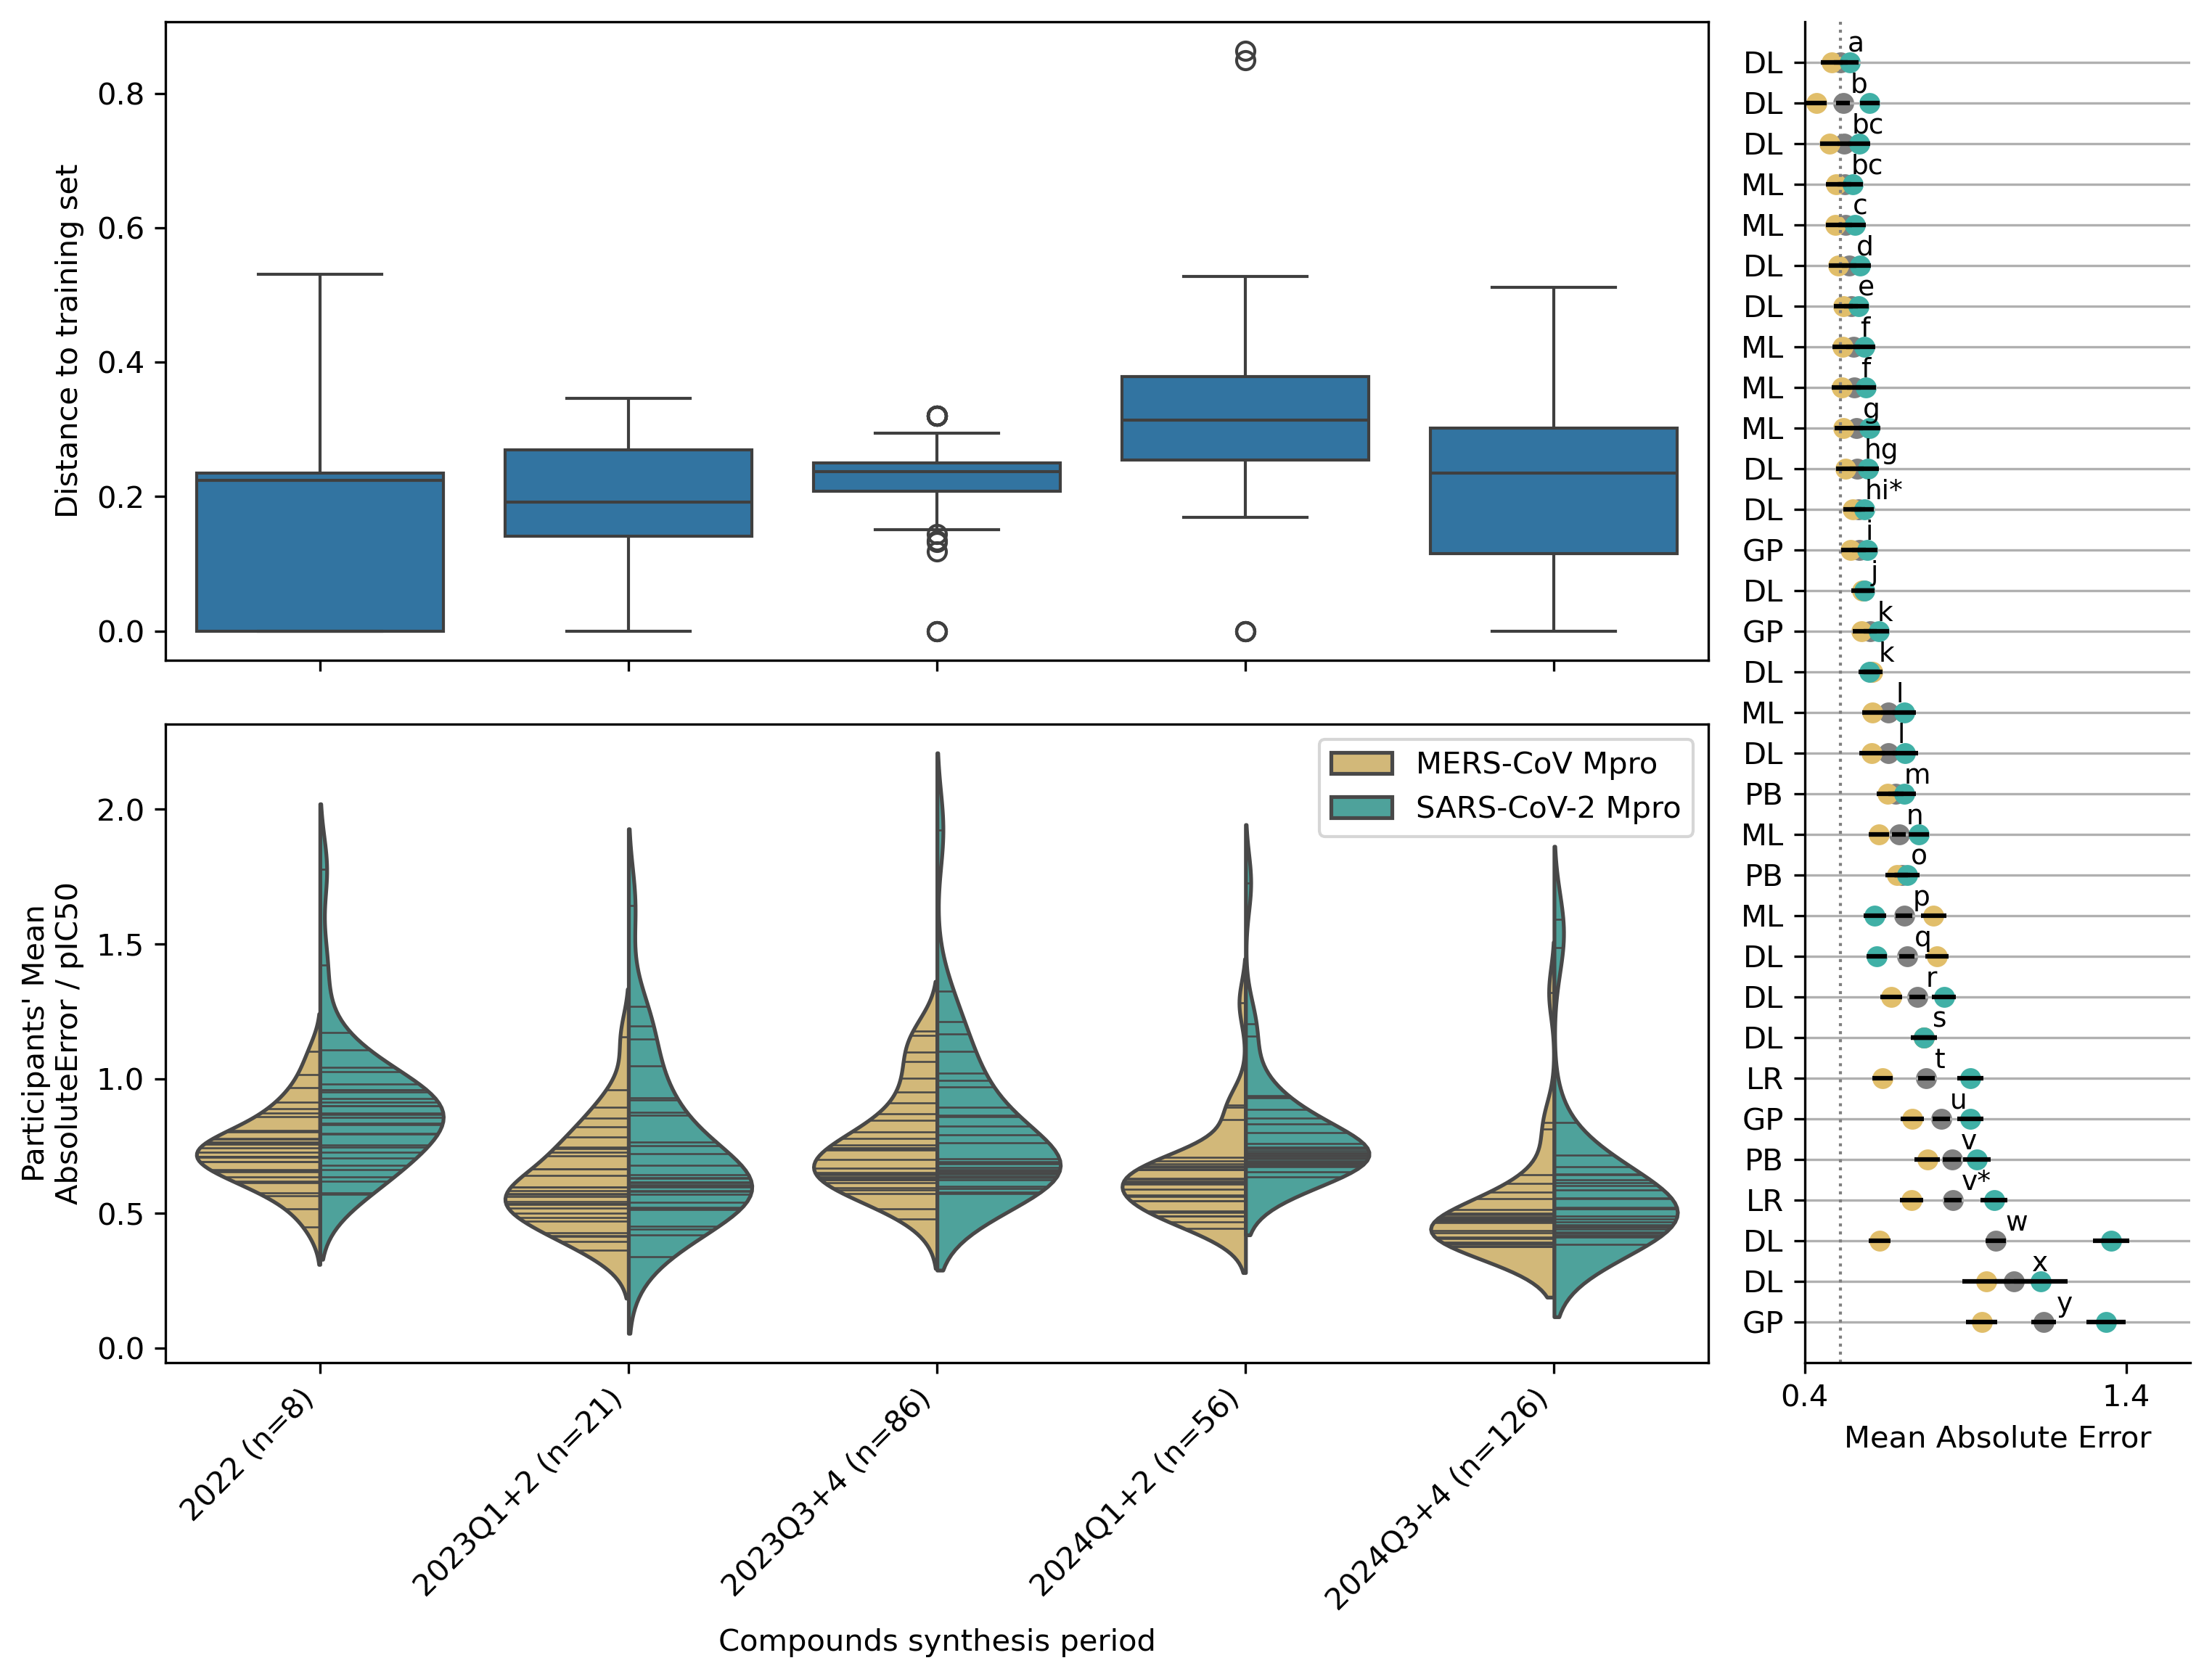
\includegraphics[scale=0.6]{04_figs_leaderboards/potency_leaderboards_and_progressions.png}
  \caption{\textbf{Participants performed diversely on ligand potency predictions for SARS-CoV-2 and MERS-CoV Mpro.} A) the Tanimoto (ECFP fingerprint) distance to the training set of compounds in the test set split by the period the compound was actioned for synthesis. B) participants' performance on each collection of compounds (as split in A) in mean absolute error of pIC50. An additional split by target (MERS-CoV Mpro in yellow, SARS-CoV-2 Mpro in green) is shown. C) leaderboard of the potency subchallenge as each entry's category (DL=Deep Learning, ML=Machine Learning, PB=Physics-Based, GP=Gaussian Process, LR=Linear Regression) and split by target in the same colors as B). Baseline models as deployed by the organizers are marked with asterisks. Each entry is annotated with its statistical ranking by the Compact Letter Display (CLD) system\cite{cld_algorithm_2004}.}
  \label{fgr:potency_leaderboards}
\end{figure}

% General description of performance %
Participants performance in the potency prediction subchallenge varied by methodology with deep learning and machine learning models outperforming physics based and other approached across the board \ref{fgr:potency_leaderboards}. Top performing entries performed well across both MERS-CoV and SARS-CoV-2 Mpro binding, with top models generally performing slightly better for the MERS-CoV endpoint relative to SARS-CoV-2. Examination of participants performance (MAE) relative to ECFP Tanimoto distances to the training set indicated that chemical similarity to the training set did not meaningfully assist model predictions across the test set. A time-wise breakdown of the test set by synthesis date also revealed limited influence of synthesis date on model performance. While general trends surrounding similarity to the training set and synthesis date could not be established, it is possible the noise from less performant models obstructs trends seen in more performant models.


% How well do people do in real terms %
Top performing participants were able to predict potency with a high degree of accuracy (macro-average MAE of 0.509 ± 0.022 for the top entry). Top performing methodologies outperformed existing graph attentional neural networks employed at ASAP to predict affinities (23rd best entry, CLD: \textit{q*}), and would have likely greatly assisted compound prioritization within our leadopt campaign. Most participants were able to outperform the ECFP linear regression baseline (29th entry, CLD: \textit{v*}) Participants ability to rank compounds by potency was also generally strong, with the top three performing entries (by primary metric MAE) displaying Kendall's $\tau$ of approximately 0.63 (mean). Note that if ordered by Kendall's $\tau$ (as with any other metric) the exact ordering within the leaderboard will shift, with general trends maintained, again highlighting the need for a holistic set of metrics rather than focus on a single one. As with the ability of these top performing models to predict absolute pIC50s to within approximately half a log unit, their ability to rank compounds by affinity was also impressive, considering that experimental potency measurement assays are expected to have significant reproduction variance. A recent study estimated approximately 1 kcal/mol (approx 0.7 pKi units)\cite{ross_maximal_2023} for a wide set of experimental measurements. Additionally, a recent study of ChEMBL\cite{landrum_combining_2024} determined Kendall's $\tau$ between rigorously curated measurements on the same set of compounds to be approximately 0.71.

% How did they do it %
Analysis of top performing affinity prediction methods reveals a diverse set of deep learning approaches including the MolE\cite{mendez-lucio_mole_2024} and MolGPS\cite{sypetkowski2024scalabilitygnnsmoleculargraphs} graph neural network (GNN) foundation models. Other highly performing approaches included using pre-computed features from representation learning models combined either with traditional ML models (e.g SVMs) or further neural network layers. Many participants also employed ensembling to improve model performance.  Importantly many of the top performing models (including all of the top 3) employed some kind of pre-training step involving large numbers of unlabeled chemical structures outside of the challenge data to develop embeddings for downstream task prediction. This is consistent with trends in other ML domains such as natural language processing\cite{radford2019language}. There were relatively few free energy calculation based entries overall compared to other challenges such as D3R\cite{parks_gaieb_chiu_yang_shao_walters_jansen_mcgaughey_lewis_bembenek_et}, likely hindered by both the multitask nature of the challenge (participants would need to first predict bound poses across two targets) and also the scale of the challenge (significant compute required to predict for $>500$ compounds).

\subsection{ADMET}
In order to compare across ADMET endpoints the endpoint MAE was normalized to the dynamic range for each endpoint (here referred to as the relative absolute error, RAE). As with the potency subchallenge model's ability to rank order compounds in the ADMET subchallenge was assessed using Kendall's $\tau$. Participants' performance varied across the endpoints with the solubility (KSOL) and LogD endpoints appearing the easiest to predict in relative terms. However when ranking ability is examined, the inability of even the best performing models to rank compounds by solubility is revealed, contrasting the excellent ranking performance of LogD models \ref{fgr:admet_endpoints}. This good performance on LogD is encouraging; the high frequency of amines with varying pKds will have complicated the training/test data in this challenge. Poor performance on solubility ranking is attributable both to the dynamic range available in the training set (most compounds fall generally into the range considered soluble, SI Figure \ref{fgr:admet_endpoints}) and also the noted difficulty of predicting solubility prospectively across several benchmarks. Given good MAE performance and poor ranking ability for the KSOL endpoint, it is likely that models are memorizing the absolute solubility of the training set, performing closer in practice to a classification model. HLM and MLM performance was similar across challenge entries with these proving to be the hardest to predict in relative (RAE) terms. Ranking performance across HLM and MLM was generally strong with top performing models achieving Kendall's $\tau$ between 0.5 and 0.6. Generally, the best performing models overall were performant across all endpoints.

% How well do people do in real terms %
There are several more considerations regarding utility of ADMET models in medicinal chemistry programs. As with solubility (see above), even relatively crude models that score high in MAE/RAE would have utility due to their ability to classify between in the cases of clearance (HLM/MLM) and permeability (e.g. distinguishing between high and low clearance fairly confidently). Although kinetic solubility (KSOL) was not ranked well by participants, it is considered a relatively fast and affordable option that would normally be used in upper tiers of the ADMET assay cascade - thermodynamic solubility is generally considered a more 'gold-standard' solubility endpoint and a subsequent blind challenge on this endpoint would be of considerable scientific use; ranking this endpoint may be more attainable as this assay is associated with less experimental variance.\cite{llompart_minoletti_baybekov_horvath_marcou_varnek_2024} Regardless, in this Mpro program there was no general concern with solubility due to the nature of the lead series. Exploring novel chemical space may have presented more challenging cases, but it is probable that most models used in this challenge would not have done well due to a lack of overlap in training space.

% clogp model used by medchemists was wildly outperformed by participants
During the Mpro program, an approximate model was used to predict clearance and permeability. It was observed that in the local chemical space there was a tight correlation between LogD and the computationally calculable ClogP. In turn, both permeability and clearance (HLM/MLM) were correlated to LogD. Thus, in this program the medicinal chemistry team used ClogP to tune clearance and permeability (it should be noted that this strategy is not applicable to every drug discovery program). As far as the authors have investigated participants' submissions, no group has used a strategy resembling this tactic. However, for this blind challenge a baseline ClogP linear regression was used and it is clearly outperformed by most participants' models especially for the permeability endpoint; such top-performing permeability models could have been pivotal in the Mpro program during its runtime. 

% How did they do it %
Analysis of top performing models again revealed a diverse set of strategies employed by the participants. Three of the top 5 participants employed variations on GNN architectures (e.g D-MPNN with Chemprop), with the majority employing multi-task learning. Similar to the potency challenge top performing models managed to bring additional data to bear either by pretraining or via incorporating relevant endpoint data directly into training. Some participants (including the top performer) employed proprietary data directly to assist them, while others used relevant public data (e.g ChEMBL) often with high levels of curation.

\begin{figure}
    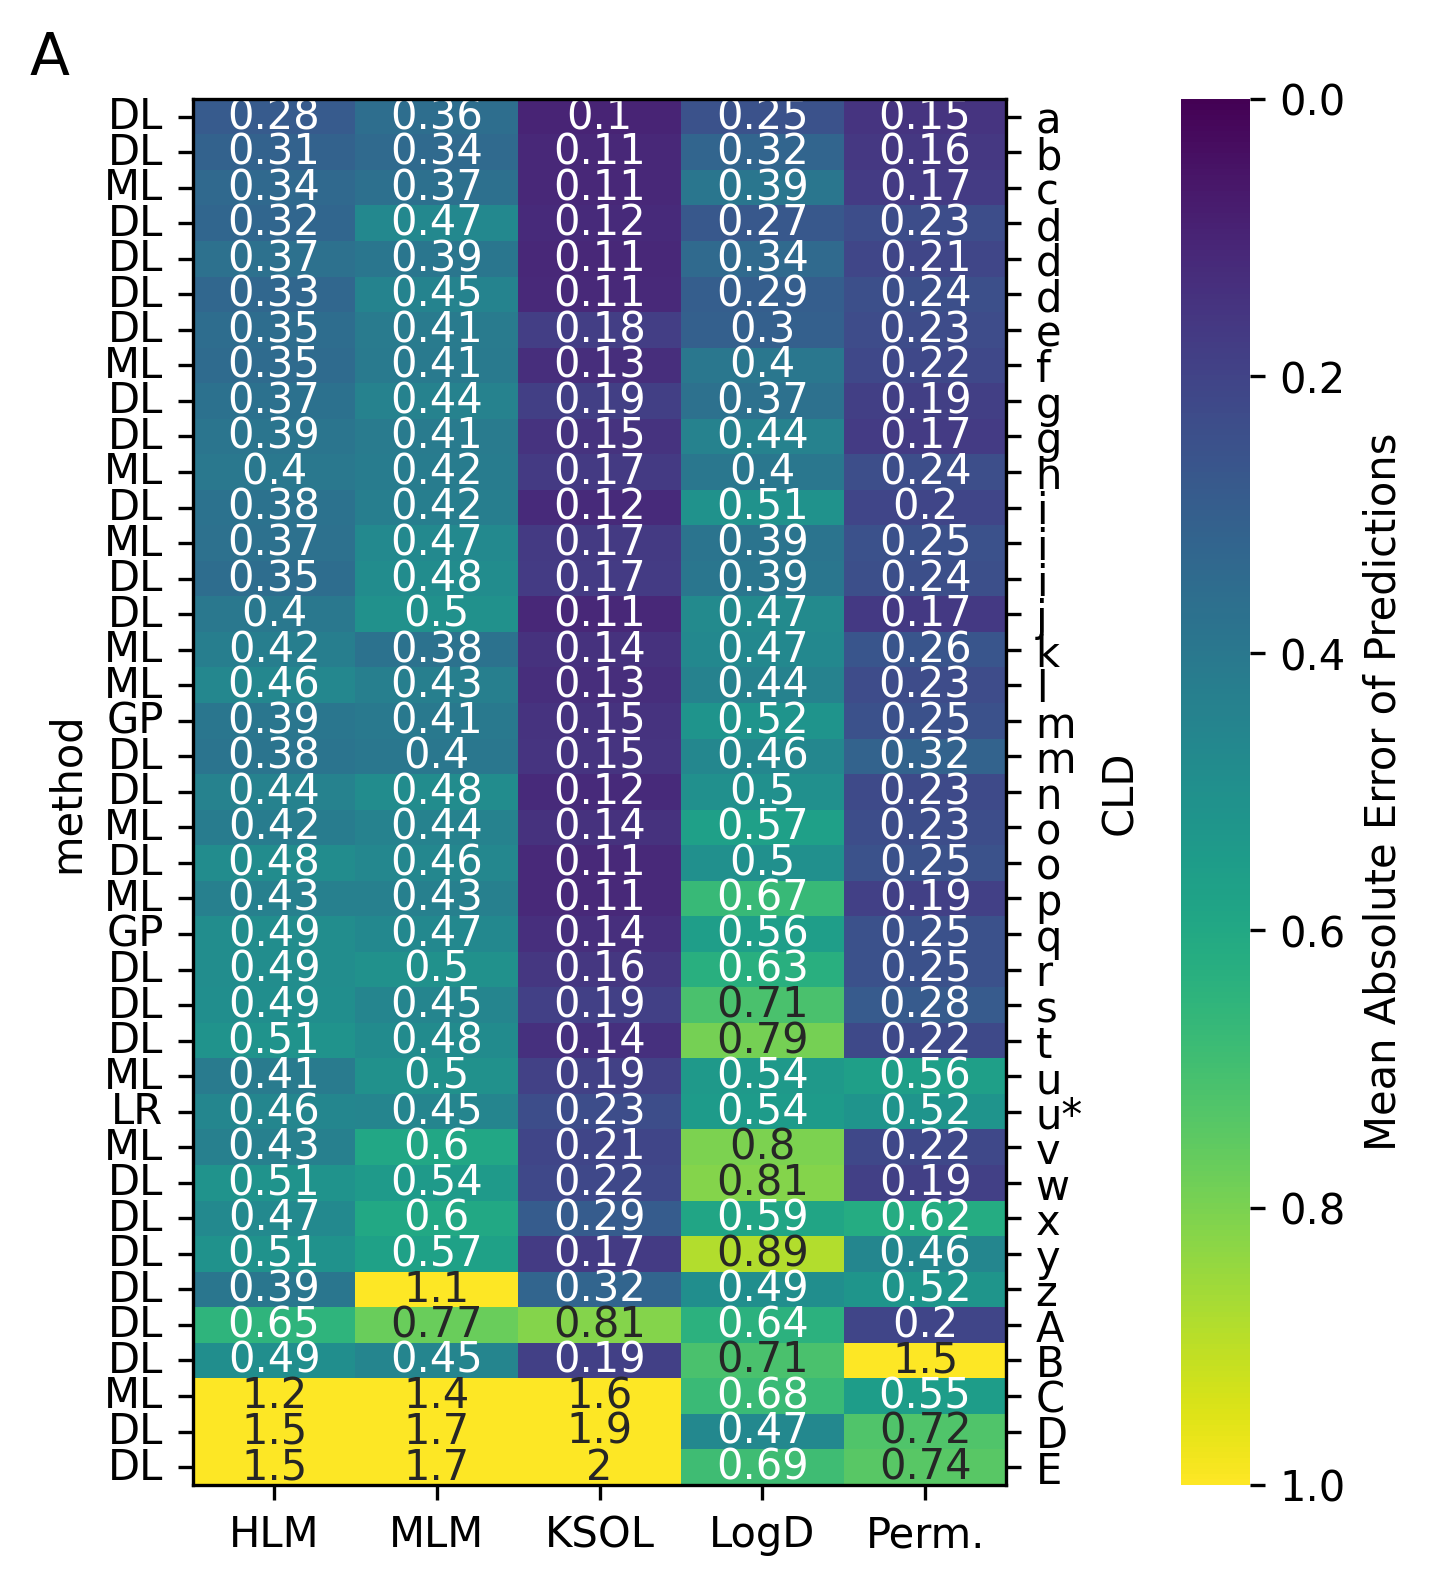
\includegraphics[scale=0.6]{fig5_admet_leaderboard/Figure_PanelA.png}
    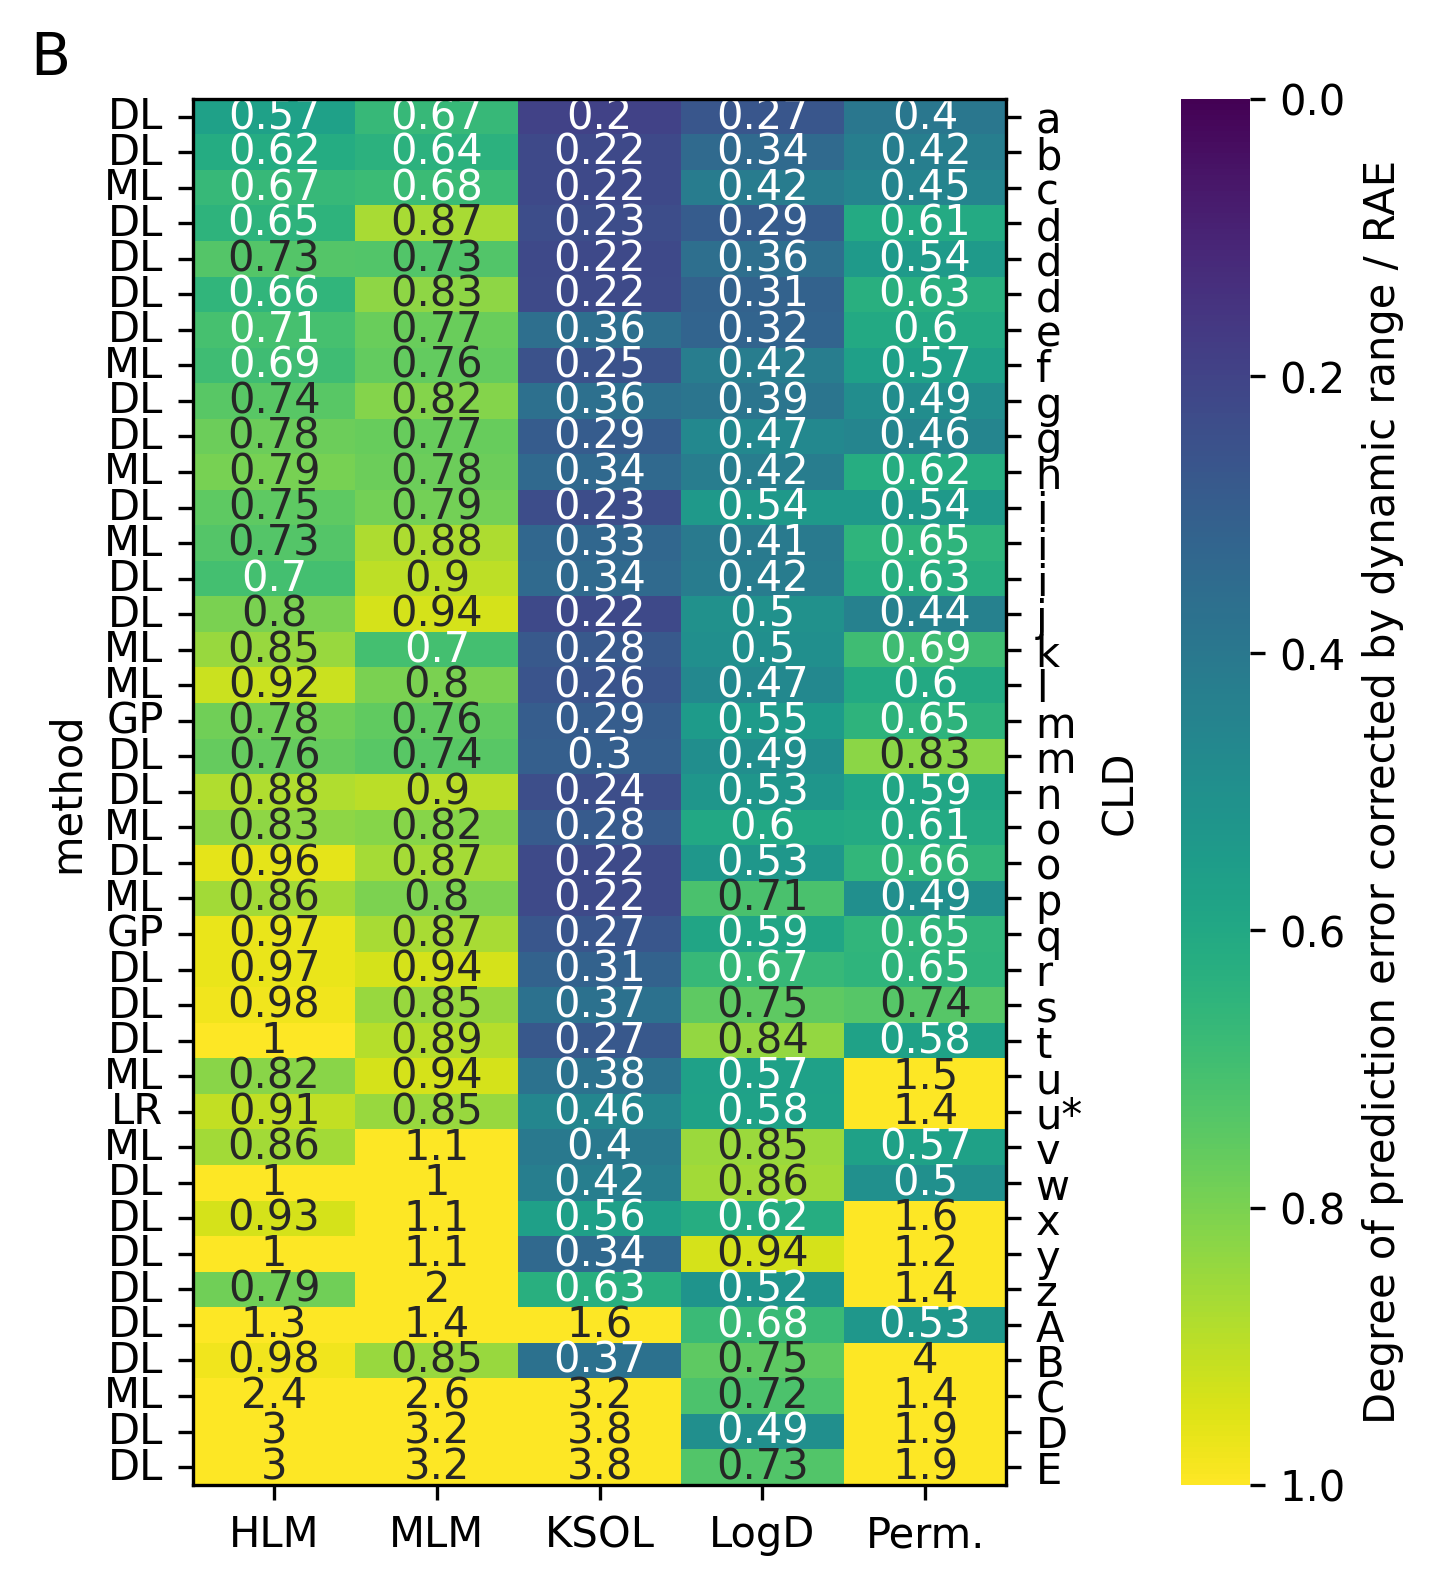
\includegraphics[scale=0.6]{fig5_admet_leaderboard/Figure_PanelB.png}
    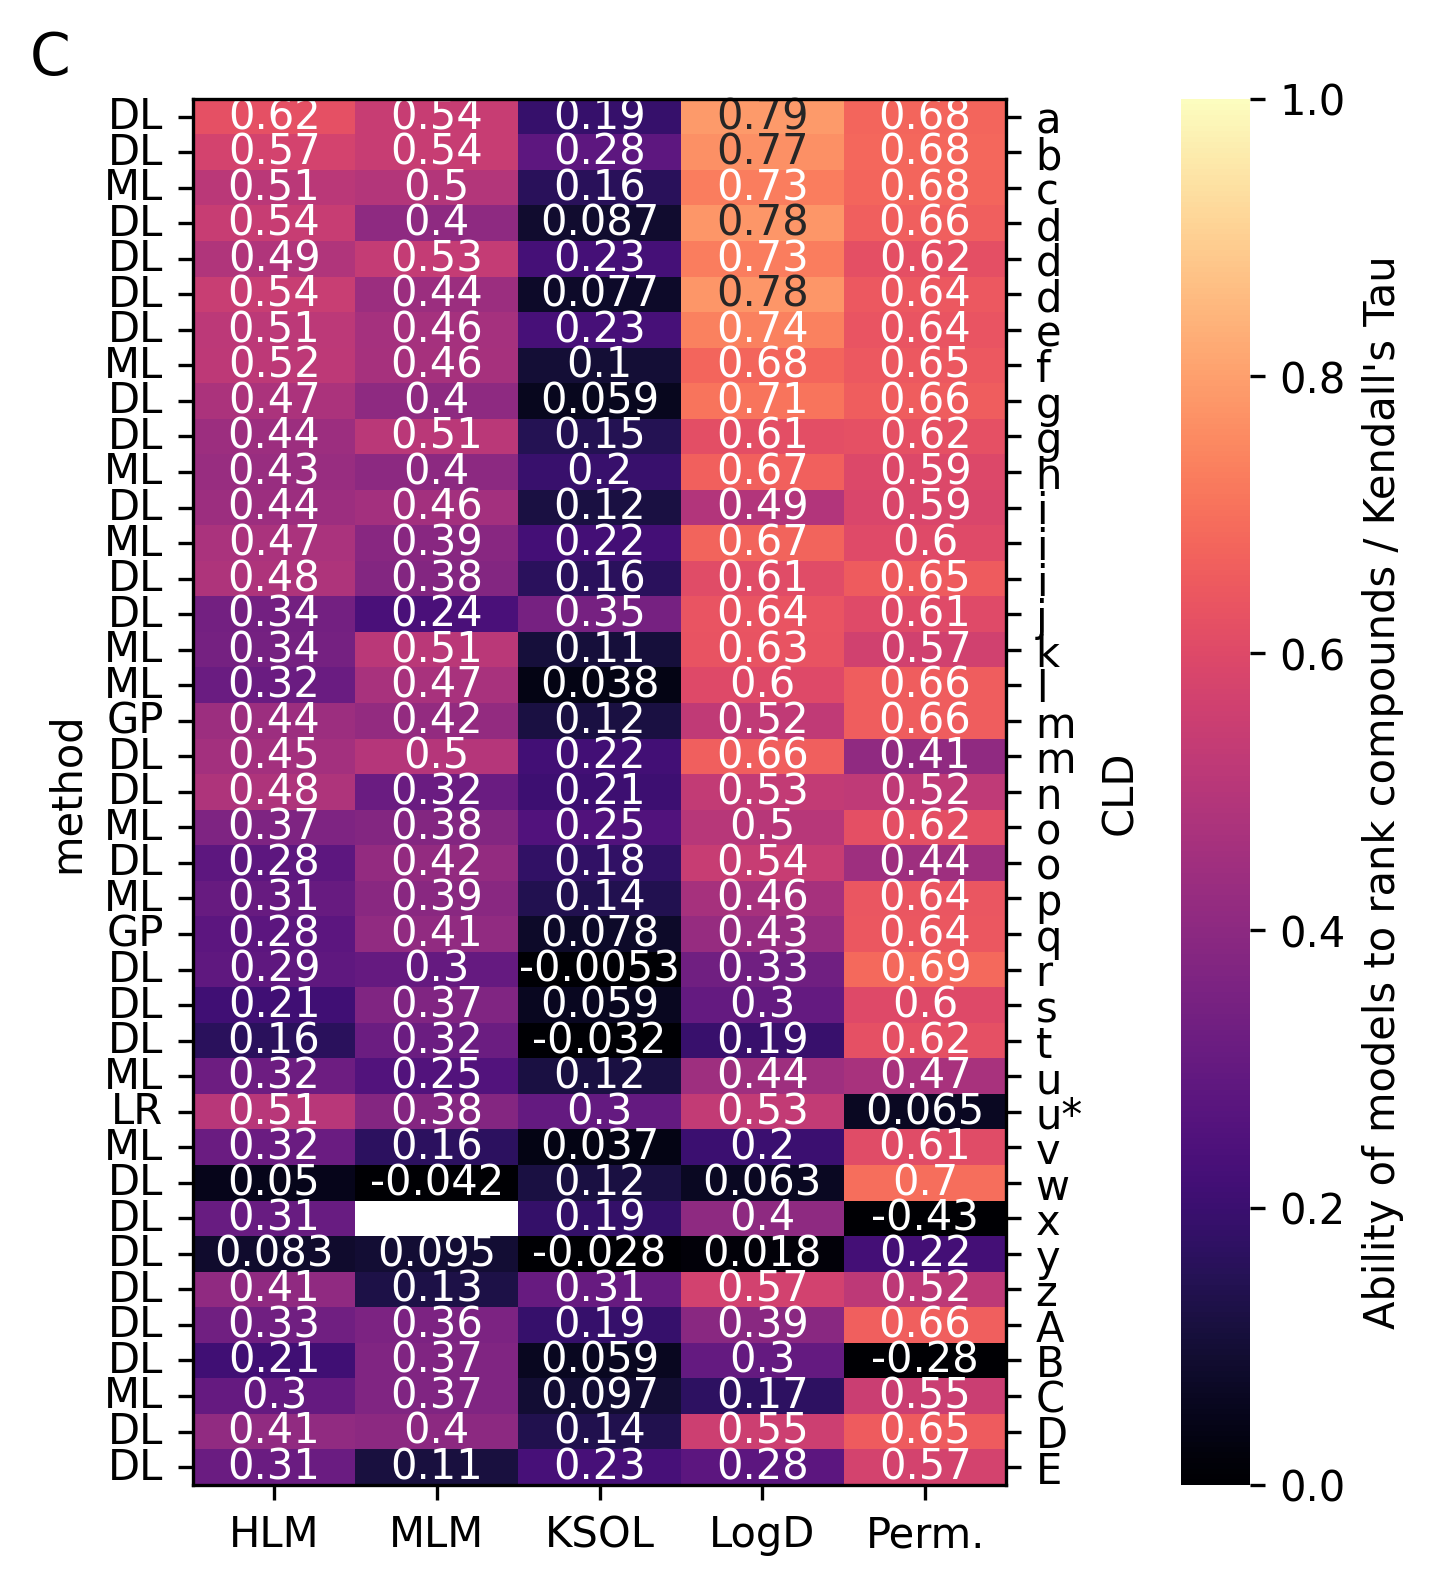
\includegraphics[scale=0.6]{fig5_admet_leaderboard/Figure_PanelC.png}
  \caption{\textbf{Participants' models performed poorly on kinetic solubility predictions but strongly on stability, permeability and lipophilicity.} Shown are (A) the mean absolute error of the normalized, predicted challenge endpoints, (B), the relative absolute error of the normalized, predicted challenge endpoints, and (C) the Kendall's $\tau$ of the normalized, predicted challenge endpoints. The empty cell at entry \textit{x} MLM consisted of constant predicted values thus no ranking coefficient was calculated. Entries are ranked by their macro-averaged MAE over all endpoints}
  \label{fgr:heatmaps_admet}
\end{figure}

\subsection{Ligand Poses}

\begin{figure}
    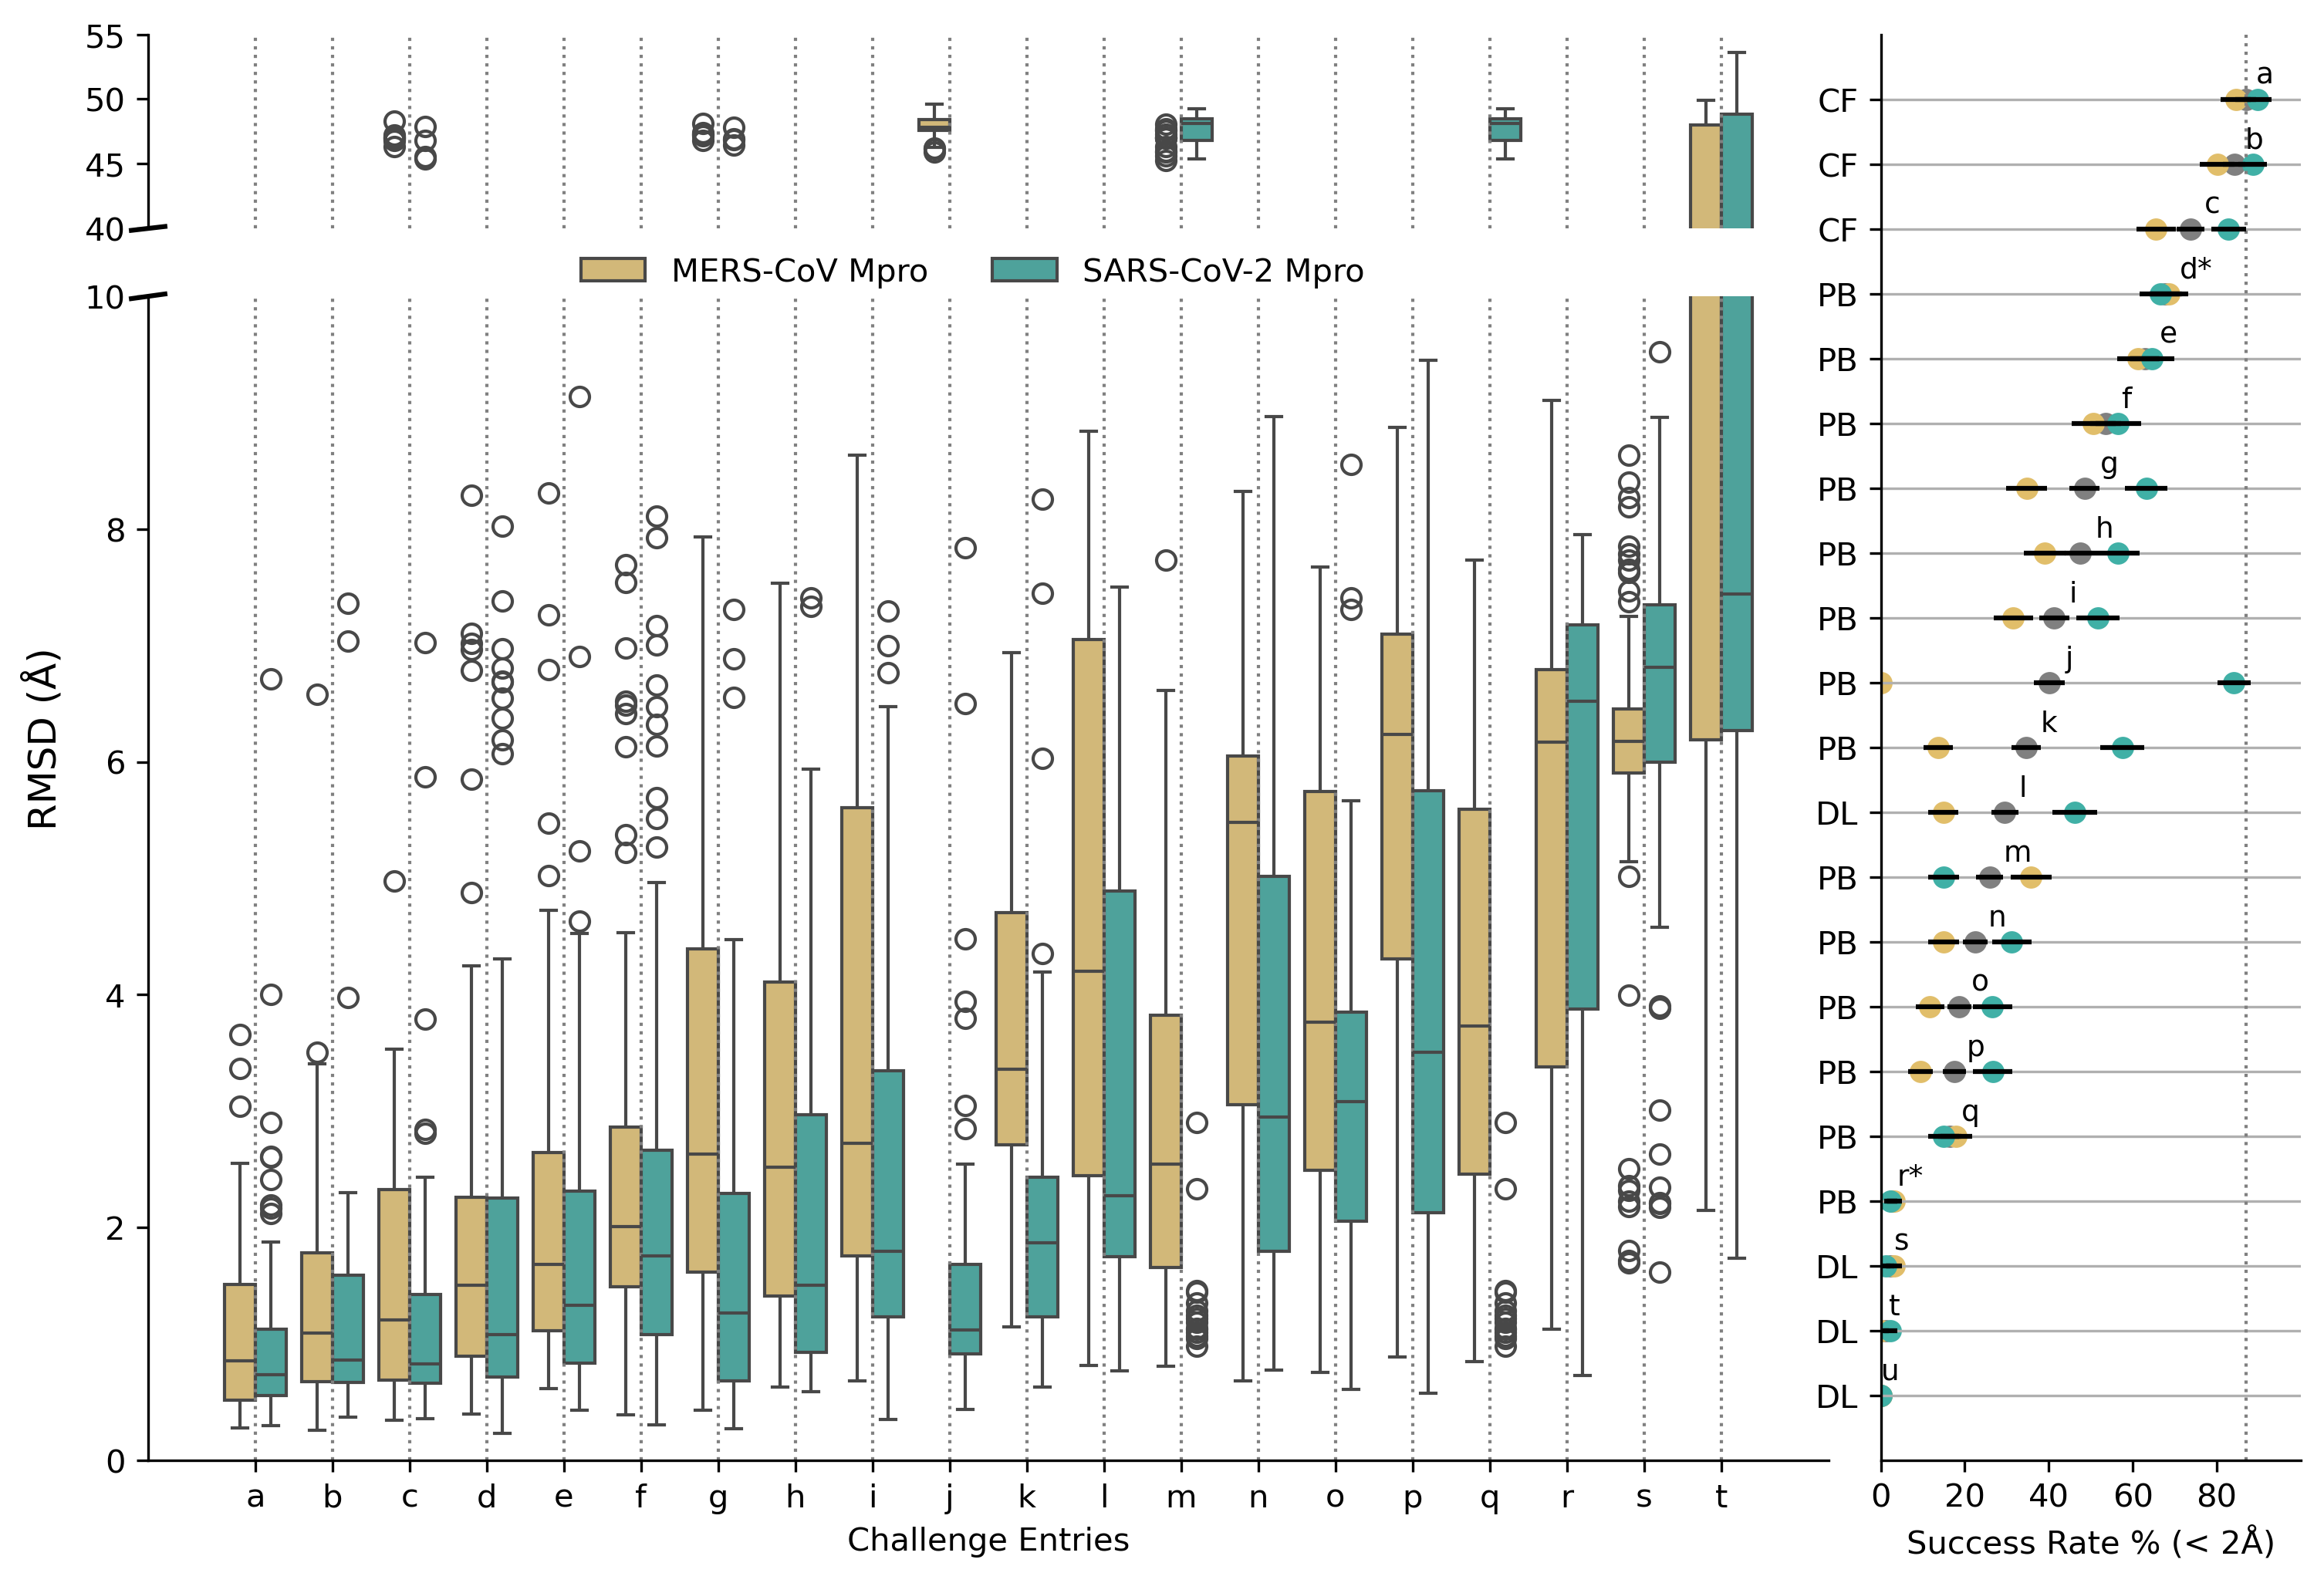
\includegraphics[width=6in
    ]{04_figs_leaderboards/pose_comp.png}
  \caption{\textbf{Participants generally performed better on the SARS-CoV-2 pose predictions than the MERS-CoV predictions, as shown by higher success rates ( ligands predicted with an RMSD \textless2Å) and lower median RMSD predictions.} Prediction RMSD distributions are shown for each entry split by the MERS-CoV and SARS-CoV-2 Mpro targets (left) with one entry removed (\textit{u}) as the full distribution lies in the axis break. The success rate of each entry is shown (right) for the overall submission (gray) and the two targets separately to further highlight the difference in performance across the targets. The overall success rate was used to determine the final ranking of the submissions.}
  \label{fgr:poses_leaderboard}
\end{figure}

Pose-prediction success was evaluated by measuring the fraction of ligands for which the predicted pose had \textless 2 Å symmetry-corrected heavy-atom RMSD from the crystallographic structure. Most participants had higher success rates for SARS-CoV-2 Mpro relative to MERS-CoV-Mpro, with an exception for \textit{m} (Figure \ref{fgr:poses_leaderboard}). When broken down by series (Figure \ref{fgr:poses_by_series_and_method} A,B) participants performed better on the lead series relative to the backup and miscellaneous series. A closer analysis shows that this trend is driven by the physics-based methods performing poorly on the backup series even when they do well on the lead series (SI Figure \ref{fgr:success_rate_lead_vs_backup}). Physics-based methods also showed the greatest discrepancy between the MERS-CoV and SARS-CoV-2 predictions, with a few of the methods showing dramatically better performance for one or the other target. Investigations of the root causes of this discrepancy is outside the scope of this work, but does highlight the sometimes idiosyncratic nature of physics based models with respect to target chemistry. 

Overall, co-folding methods performed best, including the top-performing model (\textit{a}, 82\% success rate), which far outperformed physics-based and other deep-learning-based methods (e.g deep-learning docking) in this subchallenge (Figure \ref{fgr:poses_by_series_and_method} C,D, SI Figure \ref{fgr:success_rate_lead_vs_backup}). While exciting, this likely represents high density of similar folds (high MSA depth) in the training datasets of these co-folding methods (including possible inclusion of COVID Moonshot compounds from the PDB), or subsequent fine tuning on related structures from the challenge training set, given the propensity of co-folding methods to memorize poses from their training set\cite{skrinjar_cofold_mem_2025}. In contrast to the co-folding models, all but one of the deep-learning docking methods had low success rates (with many close to 0\%), with the best performing deep-learning model (\textit{i}) having a 20\% success rate for MERS-CoV and a 40\% success rate for SARS-CoV-2 (Figure \ref{fgr:poses_leaderboard}). Given demonstrated performance of deep learning docking in other contexts and on a range of benchmarks (including in the CACHE blind challenge\cite{dunn_cache_2024}), this may represent poor sampling or be confounded by user error (including in our baseline).  Finally, the physics-based methods ranged from 0\% to 70\% success. The best performing physics-based docking method (\textit{d}) was the reference-based POSIT baseline used by the ASAP team, and the worst performing method was the non-reference-based method provided as a baseline (\textit{r}). This indicates the need for further efforts from the physics-based community with these sorts of challenges; blind challenges at this scale would likely require longer timeframes to enable this field of study to effectively participate.


\begin{figure}
    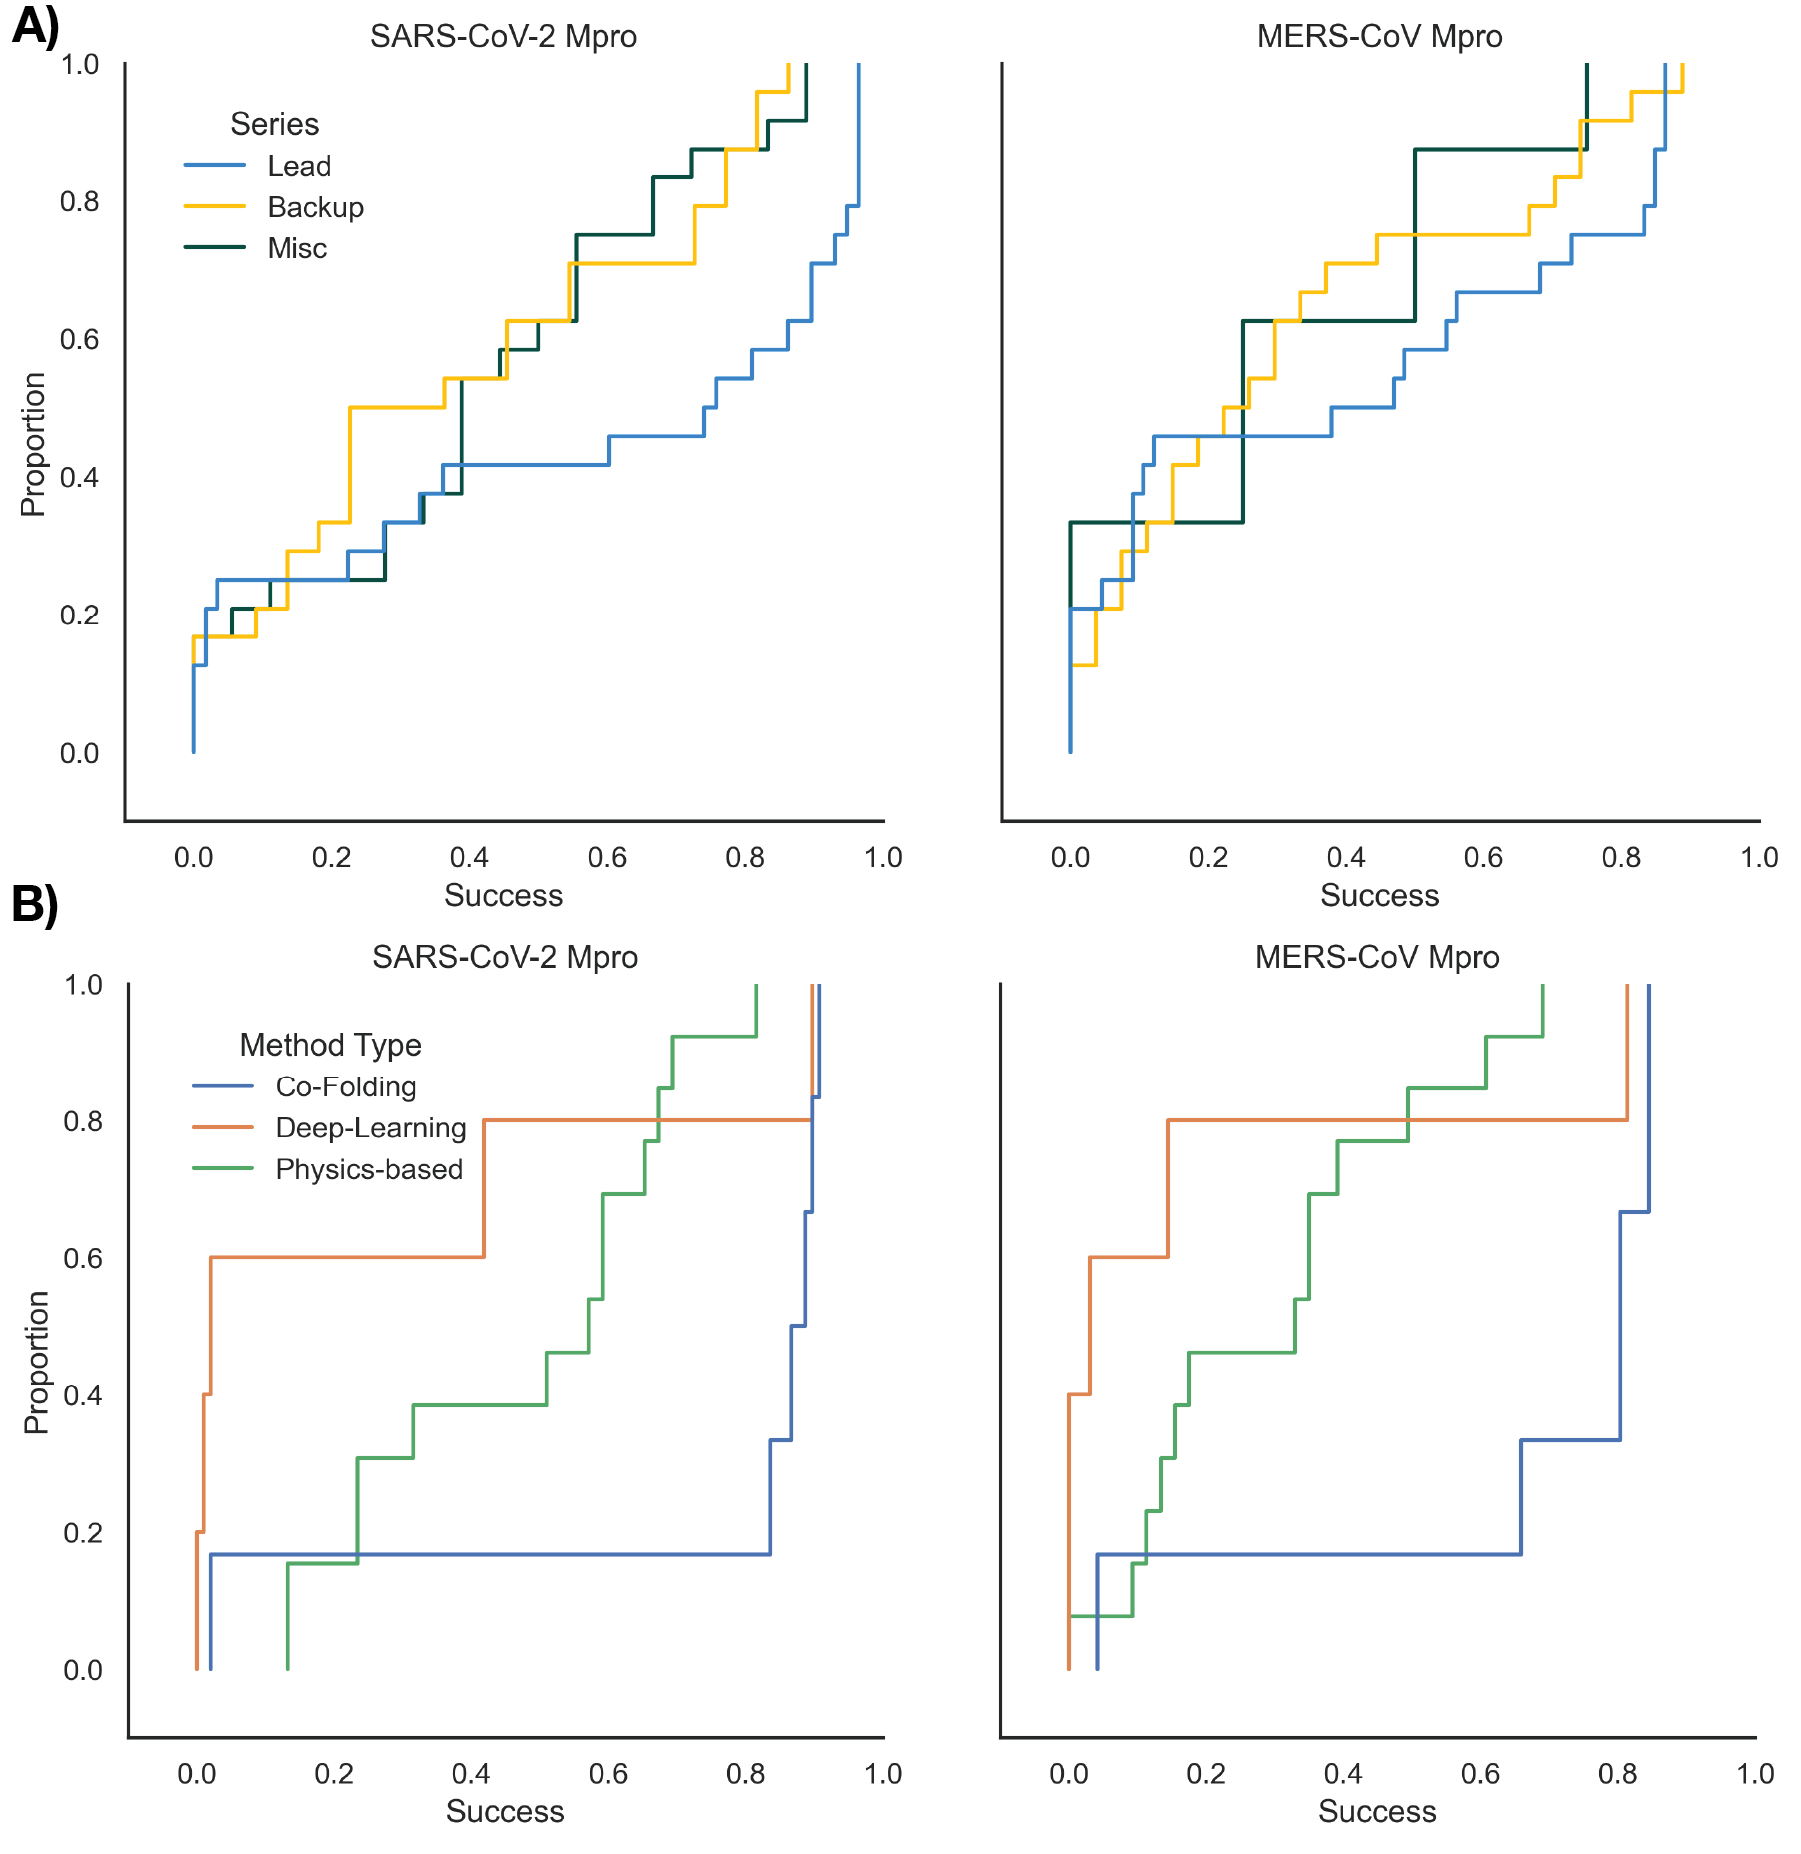
\includegraphics[scale=1
    ]{04_figs_leaderboards/poses_by_series_and_method.png}
  \caption{\textbf{Participants' performance depended on the target, series, and method type used, as shown by empirical cumulative distribution functions (ECDF) of the success rates.} The ECDF for SARS-CoV-2 (A) and MERS-CoV (B) are  split into either the lead (blue), backup (yellow), or miscellaneous (green) ligand series. Success rates are higher for the lead series than for the backup or miscellaneous series. The ECDF for SARS-CoV-2 (C) and MERS-CoV (D) are  split into the method types, either co-folding (green), deep-learning (blue), or physics-based (red). Co-folding methods perform the best, with most models exhibiting a \textgreater 80\% success rate, and deep-learning methods perform the worst, with physics-based methods exhibiting a broad range of success rates.}
  \label{fgr:poses_by_series_and_method}
\end{figure}


Predictions for this subchallenge had a large number of outliers, including conspicuous number of outliers with an RMSD of \~50 Å. In part, this stems from the design of the challenge as run through the Polaris API. As noted previously, participants uploaded the ligand pose as aligned to a reference structure. This approach was susceptible to errors, particularly when participants’ alignments to the reference structure were imperfect. This was complicated by the MERS-CoV Mpro dimer: some entries (\textit{j}, \textit{m}, \textit{q}) likely posed their entire series into the wrong chain, resulting in large errors. Additionally, for a single crystal structure in the test set, an alignment places the ligand in the wrong chain of the MERS-Cov Mpro dimer (this point was removed from analysis in this manuscript). Some participants managed to identify this issue, while others did not, highlighting the difficulty of working with data from real biological experiments.

Several of the top performing co-folding approaches employed fine-tuning on the SARS-CoV-2 Mpro structures in the training set. The \textgreater 80\% success rate of these models is impressive, and would have benefited the lead optimization of the MERS-CoV Mpro series in particular, whose structural enablement came much later in the project. These results indicate that fine-tuned co-folding models could have provided an accurate surrogate for MERS-CoV Mpro crystallography, with the caveat that a these were finetuned on large amounts of crystallography data already collected for the project.

%%%%%%%%%%%%%%%%%%%%%%%%%%%%%%%%%%%%%%%%%%%%%%%%%%%%%%%%%%%%%%%%%%%%%
%% LEARNINGS
%%%%%%%%%%%%%%%%%%%%%%%%%%%%%%%%%%%%%%%%%%%%%%%%%%%%%%%%%%%%%%%%%%%%%
\section{Challenge Key Learnings}

The ASAP-Polaris-OpenADMET blind challenge brought together participants from academia and industry around the globe to showcase cutting-edge approaches in computational methods for drug discovery on real world data. This represents a unique opportunity to gather lessons to inform future blind challenges as well as some general overarching conclusions about the performance of methodologies employed.


\subsection{Key takeaways}

% key takeaways from participants’ results
Key takeaways from the challenge include strong, across-the-board performance of neural network approaches, with these methods coming first in all three subchallenges. In the pose prediction subchallenge, cofolding and cofolding-inspired methods, such as AlphaFold-like ~\cite{abramson_2024_alphafold} and Boltz-like~\cite{wohlwend_2024_boltz-1, passaro_2025_boltz-2} architectures, significantly outperformed traditional physics-based approaches, with further improvements observed through fine-tuning. Similarly, in potency prediction, large pretrained deep learning models, especially those based on transformer and graph neural network (GNNs) architectures, were the best performers. For ADMET endpoint prediction, multi-task GNNs proved to be the best approach overall, benefiting from the ability to incorporate auxiliary data. Strong performance of top candidates is also likely in-part attributable to the focused nature of the chemical series presented in the challenge, with limited train-test distances (see Figure \ref{fgr:potency_leaderboards} A).

Notably, the top-performing approaches across the three subchallenges leveraged either auxiliary data (public or proprietary) or pre-training beyond the datasets provided by ASAP. This highlights the critical role of data availability in model performance and underscores the importance of continuing to expand open and FAIR\cite{wilkinson_fair_2016} datasets for public benefit. These findings reinforce the value of open initiatives, such as blind challenges, in providing diverse datasets for benchmarking and improving models, while also helping to establish best practices for predictive methods in drug discovery. Cutting-edge, open-science projects that may make strides in alleviating this data shortage include OpenADMET focused around ADMET properties and OpenBind focused around collecting protein structural data in high-throughput.

% Takeaways from challenge execution: Data preparation, Polaris platform, and evaluation metrics
The challenge also offered insight into strategies to successfully execute future public blind challenges. In particular, the detailed data preparation process was essential to prevent data leakage while maintaining chemical diversity, preserving real-world model applicability. Dividing the data using a temporal split in the ADMET and potency subchallenges successfully simulated a prospective drug discovery pipeline, further proving the practical relevance of the results.
Polaris proved to be an ideal platform to host a large number of participants, offering robust feedback mechanisms and enabling streamlined evaluation via a set of standardized metrics. In particular, the Python API provided an intuitive and scalable interface for handling large datasets, which facilitated broad participation. 



\subsection{Lessons learned}
The blind challenge discussed in this manuscript was designed to be a reflection of a real-world drug discovery program. With that comes intrinsic disorder that is associated with such programs, largely arising from the influx of different sources of data, different types of data, and time-dependent iteration/renewal of data. \textbf{Data preparation} for this challenge was key in ensuring smooth operation of the challenge; although a lot of effort was spent to this purpose there were still several issues found by participants throughout the runtime of the challenge. The authors note several recommendations.
\begin{enumerate}
    \item \textit{Data leakage and stereochemistry}: check carefully for train-test overlap as it can occur in many places. Particularly spend time balancing between stereo-isomers by making sure that there is an optimal distribution between AND/OR-stereochemistry mixtures. Care must be taken when working with compound registrations systems as compounds that were assayed as unresolved enantiomers may also be registered under different IDs. Crystal structures may be registered under a racemic mixture SMILES, but the resolved compound pose will typically be that of the most potent enantiomer.
    \item \textit{Data splitting}: it may not be possible to split your data points using conventional strategies. In the case of this challenge, ultimately the decision was made to settle on an \textit{index-based, time-biased} split as a compromise between several competing needs (minimal overlap, minimal cross-challenge overlap, time-wise splitting). 
    \item \textit{Data quality}: experimental data may not always be of adequate quality. Although physical activity cliffs may exist, in some cases an average measurement across replicates may be influenced by one or multiple outliers. In rare cases, dose-response curve fitting may be faulty which introduces noise into the dataset. For all these cases it is generally better to remove these data points. 
    \item \textit{Data complexity}: imbalanced distribution of the target labels can be disadvantageous to proper model training. To this end it is recommended to ensure that the distributions are overlapping between the training and test sets, and conversion to logarithmic scale should be considered as appropriate. Furthermore, assays' dynamic ranges may have been adjusted over time which can result in changing magnitudes at which measurements may be assigned as out-of-bounds. Vigilant record-keeping is helpful in this scenario, but in cases where out-of-bounds measurements were not re-measured in the new dynamic range these points may be discarded by finding their modifier (i.e., $<$, $<=$, $>=$, $>$ as opposed to $=$).
\end{enumerate}

Given adequate data preparation, \textbf{engaging the community} is required to actually run this challenge. To gather participants it is recommended to use an accessible \textbf{challenge platform} and closely \textbf{interact with the community} through social media. The authors note several recommendations.
\begin{enumerate}
    \item \textit{Programmable access to the challenge}: Programmatic API-based access to the challenge was essential to running a blind challenge successfully at this scale. Manual handling of author submissions would have proved prohibitively labor intensive and error-prone. Polaris is not the only platform that allows for this kind of challenge to be run programmatically with the  Kaggle platform very popular across the ML community (recently used successfully for a drug discovery data in the Belka challenge\cite{quigley2024belka}) with the limitation that data must fit traditional ML formats (e.g would not support protein structures). While we did run periodic evaluations (3 total) for the participants, a possible improvement for future blind challenges could be to run the evaluation in-situ following user submission to the Polaris API (as is done on Kaggle), allowing the participants to gather immediate feedback as to the performance of their models. This real-time evaluation can provide more immediate feedback as well as identify submission issues (e.g alignment issues in ligand posing subchallenge). However, this must be balanced against the possibility of exploitation of the challenge evaluation function through repeated submissions and technical feasibility of running live evaluation.
    \item \textit{Multiple sources of communication}: Our strategy of communicating with participants though multiple channels appeared successful. Discord proved a significantly helpful platform in this regard, creating a community forum for us to engage with participants and for participants to engage with each other (see Figure: \ref{fgr:timeline_engagement}). Office hours during the challenge runtime also provided a unique and valuable chance for participants to engage with experimentalists and discuss any detailed queries they might have about the provenance of the data they were building models for. The use of multiple communication channels and a social media campaign across platforms (e.g email, LinkedIn, BlueSky, X) helped build a high-quality participant base across academia and industry.
    
    \item \textit{Communicating a scope}: it is important to extensively outline the intentions and boundaries of the blind challenge \textit{a priori}. This particular challenge was unique in its realistic reflection of real-world drug discovery problems primarily in a lead optimization environment. This does entail that the chemical space is much more focussed around several similar scaffolds with small variations: several participants noted the apparent overlap in chemical space between training and test sets after observing this overlap which suggests that the challenge scope they were expecting was of a hit-to-lead/ hit discovery nature. More effective communication of this scope would have set clearer goals for this particular subset of participants.
    \item \textit{Transparency}: sharing software is key to lift the tide of computational science. For this challenge, \textit{all} software used mostly open source: this includes the leaderboard UI, submission evaluation backend and the code written to generate this manuscript. This approach, combined with ASAP Discovery's open science strategy has resulted in an exceptionally transparent blind challenge. The complete open nature of this challenge resulted in a direct feedback mechanism for participants and (not quantified) seemingly increased interest in the challenge by the community.
    \item \textit{Be open to feedback}: Throughout the process of running the challenge we received feedback on the challenge format as well as specific sub-areas (in particular the evaluation logic). This allowed us to detect and correct errors in data preparation and think more carefully about choices made in the challenge design. Expert participants can help detect issues that you may have missed or be unaware of. Long term this can contribute to a virtuous cycle of knowledge sharing in which blind challenge preparation and execution can improve over time. 
    \item \textit{Evaluation is critical}: robust evaluation of the challenge was a challenging problem given the multiple sub-challenges and the multiple endpoints within each one. Importantly, we followed a robust statistical analysis plan in which hypothesis testing was conducted to determine if model performance was statistically distinct\cite{ash_practically_2024}.  Choice of metrics and evaluation procedure has to balance interpretability against rigorous evaluation. In our case this necessitated some tradeoffs, particular for the ADMET sub-challenge. Macro-averaged MAE was chosen as a generally applicable metric, however with the drawback that for subchallenges with multiple endpoints (e.g HLM, MLM, etc for ADMET subchallenge) each endpoint contributes differently to the macro average depending on its log-normalized dynamic range.  We decided that simplicity of using macro-averaging was preferable to developing a custom analysis workflow depending on dynamic range or other approach (e.g multi-parameter optimization or ranking algorithm). This should likely be revisited for future blind challenges. Regardless, we reported multiple metrics such that participants could draw their own conclusions about model performance from the full leaderboard.
    \item \textit{Continue the conversation}: after the challenge ended, there was a sense of collaboration between the participants - predictions were compared and certain datapoints were discussed in detail as the datasets were unblinded after the final submission date. Using this momentum, several seminars were hosted where top performers were given the opportunity to present their methodology and learnings. The unblinded challenge dataset as well as the Discord channel remain open to this day and offer an effective forum for novel science in molecular modeling.
\end{enumerate}


\subsection{The future of blind challenges}

% Outlook for future challenges
We believe that blind challenges are the best way to robustly assess models and to advance computational methods in drug discovery. This is validated by step-change improvements in model performance after community investment in blind challenges both in related fields such as computer vision (ILSVRC\cite{ILSVRC15}, COCO\cite{coco}, ISIC\cite{tschandl_humancomputer_2020}, Vesuvius Challenge\cite{vesuvius}) and natural language processing (GLUE\cite{wang2019gluemultitaskbenchmarkanalysis}, SuperGlue\cite{sarlin2020supergluelearningfeaturematching},  SQuAD\cite{rajpurkar2016squad100000questionsmachine}), and in those relevant to drug discovery such as computational structure prediction (CASP)\cite{casp13_2019, casp14_2021, casp15_2023}. For blind challenges to become a successful measuring stick around which a field gathers, several pillars need to be addressed. Firstly, high-quality realistic datasets need to be used or generated, representing a realistic use case on which models would be expected to perform in production. Secondly, challenges need to be "industrialized" in execution, with high-quality infrastructure, allowing blind challenges to be more routine, consistent, and operate with lower overhead. Finally, an iterative cycle of improvement must be fostered, in which community engagement drives iterative improvement in model performance. Open-source code and datasets are critical to this endeavor, allowing continual engagement and retrospective performance analysis around which the community can gather. 

John and Jamie to expand: XXXXX



\section{Acknowledgments}

The authors thank the participants, as well as supporting staff at the primary institutions involved (ASAP Discovery, Open Molecular Software foundation, Valence Labs, UCSF) and Dr David Mobley for valuable discussions and feedback on running computational blind challenges. Special thanks go to the experimentalists across the ASAP Discovery Consortium without whom the challenge would not have been possible. 

\section{Funding}

% OpenADMET
Research reported in this publication was partially supported by the Advanced Research Projects Agency for Health (ARPA-H) under AVOID-OME: Structurally enabling the “avoid-ome” to accelerate drug discovery, and Award Number 1AY1AX000035-01. The ARPA-H award provided XX\% of total costs and total XX \% [Award Recipient must identify percentage of total award costs and total award dollars]. The contents are those of the author. They may not reflect the policies of the Department of Health and Human Services or the U.S. government. The content is solely the responsibility of the authors and does not necessarily represent the official views of the Advanced Research Projects Agency for Health.\
% ASAP 
Research reported here was supported in part by NIAID of the National Institutes of Health under award number U19AI171399.
% John D. Chodera
John D.\ Chodera acknowledges support from NIH/NCI Cancer Center Support Grant P30 CA008748 and the Sloan Kettering Institute.

\section{Disclaimers}
% ASAP
The content is solely the responsibility of the authors and does not necessarily represent the official views of the National Institutes of Health.

\section{Disclosures}
% John D. Chodera
John D.\ Chodera is a current member of the Scientific Advisory Board of OpenEye Scientific Software, and is co-Founder, President, and CEO and has equity interests in Achira Inc.
A complete funding history for the Chodera lab can be found at \url{http://choderalab.org/funding}.


%%%%%%%%%%%%%%%%%%%%%%%%%%%%%%%%%%%%%%%%%%%%%%%%%%%%%%%%%%%%%%%%%%%%%
%% The same is true for Supporting Information, which should use the
%% suppinfo environment.
%%%%%%%%%%%%%%%%%%%%%%%%%%%%%%%%%%%%%%%%%%%%%%%%%%%%%%%%%%%%%%%%%%%%%
\begin{suppinfo}

Additional analyses to support main conclusions. 

\end{suppinfo}

%%%%%%%%%%%%%%%%%%%%%%%%%%%%%%%%%%%%%%%%%%%%%%%%%%%%%%%%%%%%%%%%%%%%%
%% The appropriate \bibliography command should be placed here.
%% Notice that the class file automatically sets \bibliographystyle
%% and also names the section correctly.
%%%%%%%%%%%%%%%%%%%%%%%%%%%%%%%%%%%%%%%%%%%%%%%%%%%%%%%%%%%%%%%%%%%%%
\bibliography{references}

\end{document}